\documentclass[aspectratio=169]{beamer}
\beamertemplatenavigationsymbolsempty
\usetheme{Madrid}
\usecolortheme{default}
\setbeamertemplate{navigation symbols}{}
\definecolor{sectionblue}{rgb}{0,0.1,0.4}
% \documentclass{beamer}
\usepackage{listings}
\usepackage[T1]{fontenc} % Often helpful for typesetting special characters like _ directly in \texttt
\usepackage[utf8]{inputenc} % If using UTF-8 characters
\usepackage{graphicx, hyperref, amsmath, animate, tabularx, bm, amssymb, amsfonts, float}
\usepackage{tikz} % For diagrams
\usetikzlibrary{shapes, arrows, positioning, fit, calc}
\usepackage{booktabs} % For professional quality tables
\usepackage{adjustbox} % To resize table if needed
\usepackage{mathtools}
\usepackage{algorithm}
\usepackage[noend]{algpseudocode}
\usepackage{breqn}
\usepackage{hyperref}
\usecolortheme{beaver}
\usefonttheme{professionalfonts}
\graphicspath{{Figures/}}
\usepackage{listings} % For code/log snippets

\usepackage[backend=biber, style=authortitle, sorting=none,
autocite=footnote, citetracker=false, ibidtracker=false]{biblatex}
\addbibresource{ref.bib}
\renewcommand*{\bibfont}{\scriptsize}

\DeclareFieldFormat{title}{\textcolor{blue}{\mkbibquote{#1\isdot}}}
\DeclareFieldFormat{citetitle}{\textcolor{blue}{\mkbibquote{#1\isdot}}}
\DeclareFieldFormat{titlecase}{\textcolor{blue}{#1}}
\DeclareFieldFormat[article,inproceedings,incollection,thesis,unpublished]{title}{\textcolor{blue}{\mkbibquote{#1\isdot}}}
\DeclareFieldFormat[article,inproceedings,incollection,thesis,unpublished]{citetitle}{\textcolor{blue}{\mkbibquote{#1\isdot}}}
\DeclareFieldFormat[book,misc,online,report,inbook]{title}{\textcolor{blue}{\emph{#1}}}
\DeclareFieldFormat[book,misc,online,report,inbook]{citetitle}{\textcolor{blue}{\emph{#1}}}

% Keep footnotes compact: author + short title + year only
\AtEveryCitekey{%
	\clearfield{pages}\clearfield{volume}\clearfield{number}%
	\clearfield{doi}\clearfield{url}\clearfield{eprint}\clearfield{eprinttype}%
	\clearfield{note}\clearfield{isbn}\clearfield{issn}%
}

\setbeamerfont{footnote}{size=\tiny}

\usepackage{listings}
\usepackage{xcolor}

\newcommand{\ttitle}{Cross-Lingual Mechanisms in Multilingual Language Models and Reinforcement Learning}
\newcommand{\tdate}{June 29, 2026}

% \definecolor{codegreen}{rgb}{0,0.6,0}
% \definecolor{codegray}{rgb}{0.5,0.5,0.5}
% \definecolor{codepurple}{rgb}{0.58,0,0.82}
% \definecolor{backcolour}{rgb}{0.95,0.95,0.92}

% \lstdefinestyle{mystyle}{
	%     backgroundcolor=\color{backcolour},   
	%     commentstyle=\color{codegreen},
	%     keywordstyle=\color{magenta},
	%     numberstyle=\tiny\color{codegray},
	%     stringstyle=\color{codepurple},
	%     basicstyle=\ttfamily\footnotesize,
	%     breakatwhitespace=false,         
	%     breaklines=true,                 
	%     captionpos=b,                    
	%     keepspaces=true,                 
	%     numbers=left,                    
	%     numbersep=5pt,                  
	%     showspaces=false,                
	%     showstringspaces=false,
	%     showtabs=false,                  
	%     tabsize=2,
	% }

% \lstset{style=mystyle}
\renewcommand*{\bibfont}{\scriptsize}
\newcommand{\pref}{\succ} % Define preference symbol
\newcommand{\Tref}{\pi_{\mathrm{ref}}} % Reference policy
\newcommand{\pith}{\pi_{\theta}} % Policy theta
\newcommand{\rphi}{r_{\phi}} % Reward phi
\newcommand{\Dprefs}{\mathcal{D}_{\text{prefs}}} % Preference dataset
\newcommand{\Exp}{\mathbb{E}} % Expectation
\newcommand{\sig}{\sigma} % Sigmoid
\newcommand{\Dg}{\mathcal{D}_g} % Group dataset
\newcommand{\E}{\mathbb{E}}
\newcommand{\R}{\mathbb{R}}
\DeclareMathOperator*{\argmax}{arg\,max}
\DeclareMathOperator*{\argmin}{arg\,min}
\newcommand{\dataset}{\mathcal{D}}
\newcommand{\labels}{\mathcal{T}} % Set of all T labels
\newcommand{\privileged}{\mathcal{P}} % Privileged label set
\newcommand{\nonprivileged}{\bar{\mathcal{P}}} % Non-privileged label set
\newcommand{\confusing}{S_{il}} % Confusing set for instance i, label l
\newcommand{\model}{m} % Model function for scores/logits
\newcommand{\params}{\mathbf{w}} % Model parameters
\newcommand{\Params}{\{\mathbf{w}_t \vert \exists t \in \mathcal{T}\}} % Model parameters
\newcommand{\refparams}{\hat{\mathbf{w}}} % Reference model parameters
\newcommand{\Refparams}{\{\hat{\mathbf{w}}_t \vert \exists t \in \mathcal{T}\}} % Model parameters
\newcommand{\loss}{\mathcal{L}}
\newcommand{\baseloss}{\ell} % Base classification loss (e.g., BCE)
\newcommand{\policy}{\pi}
\newcommand{\refpolicy}{\pi_{\mathrm{ref}}}
\newcommand{\attributes}{\mathcal{A}}
\setbeamerfont{footnote}{size=\tiny}

% --- FONT SIZE CUSTOMIZATIONS ---
% Set the font for block titles (all types) and captions to scriptsize globally
\setbeamerfont{block title}{size=\scriptsize}
\setbeamerfont{block title alerted}{size=\scriptsize} % For alertblock titles
\setbeamerfont{block title example}{size=\scriptsize} % For exampleblock titles
\setbeamerfont{caption}{size=\scriptsize}
\setbeamerfont{caption name}{size=\scriptsize} % For "Figure X:" part of caption
\setbeamerfont{footnote}{size=\tiny}

\title[MS by Research: Thesis Defence]{\ttitle}
\author[Soumen Mondal]{\textcolor{blue}{Soumen Kumar Mondal} \\\texttt{23m2157@iitb.ac.in}}
\institute[IIT Bombay]{\textcolor{blue}{Supervisor: Prof.~Preethi Jyothi, CSE, IIT Bombay\\External Examiner: Prof.~Pawan Goyal, CSE, IIT Kharagpur\\Internal Examiner \& Chairman: Prof.~Biplab Banerjee, CSRE, IIT Bombay}\\\;\\MS by Research in Data Science and Artificial Intelligence\\Center for Machine Intelligence and Data Science (CMInDS)\\Indian Institute of Technology Bombay, Mumbai, India}
\date{\tdate}

%========================================================================
%  PART-DIVIDER FRAME
%  A centered frame showing only the part title (no frametitle/subtitle).
%  Reuse this for: Introduction, Part 1, Part 2, Part 3, Conclusion.
%========================================================================
\newcommand{\partdivider}[2]{%
	\begin{frame}
		\vspace*{\fill}
		\begin{center}%
			\begin{minipage}{0.9\textwidth}
				\begin{beamercolorbox}[rounded=true,shadow=true,sep=18pt,center]{block body}
					{\color{sectionblue}\Large\textbf{#1}}\\[0.6em]
					{\color{black!70}\normalsize #2}
				\end{beamercolorbox}
			\end{minipage}%
		\end{center}
		\vspace*{\fill}
	\end{frame}%
}

\begin{document}
	% Title page frame
	\begin{frame}
		\titlepage
	\end{frame}
	
	
	%========================================================================
	%  INTRODUCTION
	%========================================================================
	
	\partdivider{Introduction}{Motivation, Problem Setting, and Research Questions}
	
	% --- Intro Slide 1: Motivation & Problem ---
	\begin{frame}{Introduction}
		\framesubtitle{Motivation and Problem Setting}
		\begin{block}{\scriptsize Motivation}\scriptsize
			\begin{itemize}
				\item Large language models use the same parameters across languages, but perform worse on low-resource languages \autocite{conneau2018xnli, shi2022mgsm}.
				\item It is difficult to identify which part of a model is responsible for a behaviour, and difficult to change that behaviour by editing a specific part.
				\item This thesis presents three studies, examining where a capability is located inside a model and how training shapes the model's behaviour:
				\begin{itemize}\scriptsize
					\item Language-specific neurons and cross-lingual transfer in multilingual language models. \hfill (Part 1)
					\item Cross-lingual behaviour during reinforcement-learning fine-tuning of a multilingual reasoner. \hfill (Part 2)
					\item Training with competing objectives in multi-label classification. \hfill (Part 3)
				\end{itemize}
			\end{itemize}
		\end{block}
		
		\begin{block}{\scriptsize Problem Setting}\scriptsize
			\begin{itemize}
				\item Each study asks where a behaviour can be changed: by editing a localized component, or through training.
				\item Part 1 edits components, Part 2 observes a training procedure, and Part 3 designs an objective.
			\end{itemize}
		\end{block}
	\end{frame}
	
% --- Intro Slide: Research Questions ---
\begin{frame}{Introduction}
	\framesubtitle{Research Questions}
	\begin{block}{\scriptsize Questions Addressed in This Thesis}\scriptsize
		\begin{enumerate}
			\item Are language-specific neurons useful for cross-lingual transfer?
			Earlier work shows they can control the language a model generates in \autocite{tang2024language}. We test whether editing them improves downstream performance on tasks such as NLI and QA for low-resource languages, not only the language of generation. \hfill (Part 1)
			\item Does a multilingual model process its reasoning in English at the middle layers, and is that what holds back low-resource languages?
			One hypothesis is that the model works in an English-leaning space at the middle layers \autocite{wendler2024llamas}. We track a model during reinforcement-learning fine-tuning to see whether this holds, and identify the factor that controls why some languages improve and others do not. \hfill (Part 2)
			\item Can preference optimization, which was developed for text generation, manage competing objectives in classification?
			We test whether the ideas in DPO \autocite{rafailov2023direct}, CPO \autocite{xu2024contrastive}, and SimPO \autocite{meng2024simpo}, with a group-robust balancing method \autocite{ramesh2024group}, improve a chosen subset of labels while keeping performance on the rest stable. \hfill (Part 3)
		\end{enumerate}
	\end{block}
\end{frame}
	
	% --- Intro Slide 4: A Note on Naming ---
	\begin{frame}{Introduction}
		\framesubtitle{Note on the Abbreviation GRPO}
		\begin{block}{\scriptsize Two Methods with the Same Abbreviation}\scriptsize
			\begin{itemize}
				\item Two methods in this thesis share the abbreviation GRPO:
				\begin{itemize}\scriptsize
					\item Part 2: Group Relative Policy Optimization \autocite{shao2024deepseekmath}, a reinforcement-learning algorithm.
					\item Part 3: Group Robust Preference Optimization \autocite{ramesh2024group}, a method from robust optimization used to balance the two label groups in FairPO.
				\end{itemize}
				\item The full name is written out in each part, and the abbreviation alone is not used to refer to either.
			\end{itemize}
		\end{block}
	\end{frame}
	
	
	%========================================================================
	%  PART 1 : LANGUAGE-SPECIFIC NEURONS
	%========================================================================
	
	\partdivider{Part 1}{Language-Specific Neurons Do Not Facilitate Cross-Lingual Transfer}
	
	% ----------------------------------------------------------------------
	% Slide 4: Definition of a Neuron
	% ----------------------------------------------------------------------
	\begin{frame}{Part 1: Language-Specific Neurons}
		\framesubtitle{Definition of a Neuron}
		\begin{columns}
			\column{0.5\textwidth}
			\begin{block}{\scriptsize Neuron as an Activation Dimension}\scriptsize
				\begin{itemize}
					\item A neuron is one dimension of the MLP activation vector $\mathbf{h}^i$:
					\begin{equation}
						\mathbf{h}^i = [ \text{act\_fn}(\hat{\mathbf{H}}^i \mathbf{W}_1^i) \otimes (\hat{\mathbf{H}}^i \mathbf{W}_3^i) ] \cdot \mathbf{W}_2^i.
					\end{equation}
					\item Its average activation over token positions, measured on Wikipedia text, is
					\begin{equation}
						\bar{h}_{i,j} = \frac{1}{T} \sum_{t=1}^{T} h_{i,j}^t.
					\end{equation}
				\end{itemize}
			\end{block}
			\column{0.4\textwidth}
			\begin{block}{\scriptsize MLP Block in Llama 3}\scriptsize
				\begin{figure}
					\centering
					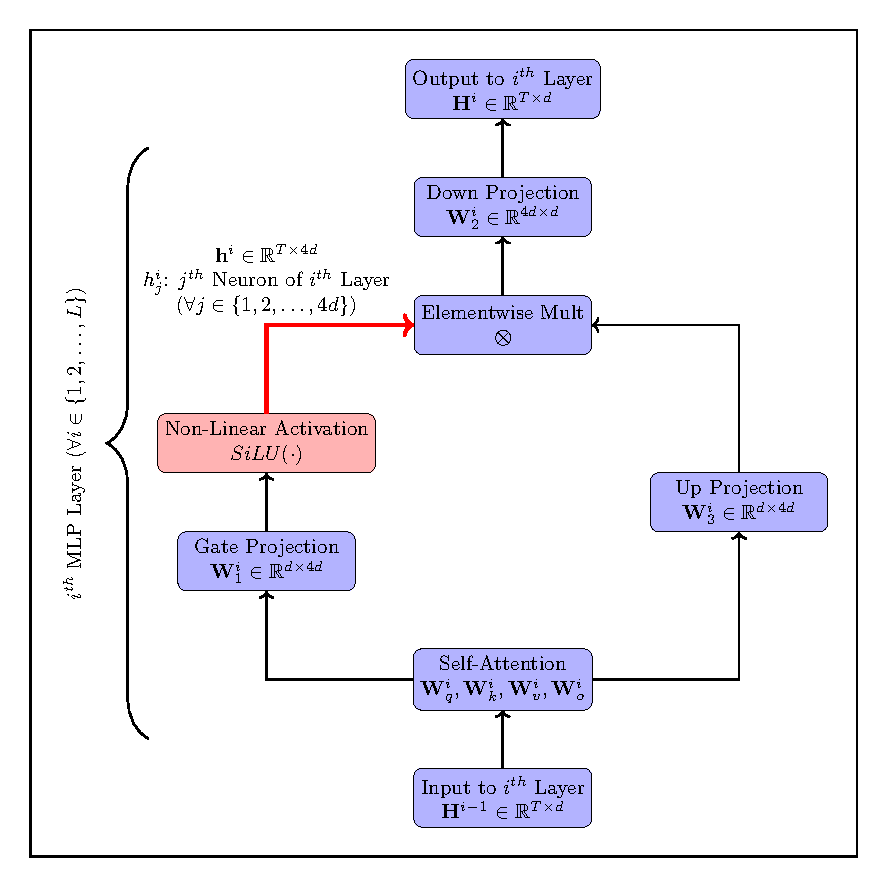
\includegraphics[width=0.9\textwidth]{mlp.pdf}
				\end{figure}
			\end{block}
		\end{columns}
	\end{frame}
	
	% ----------------------------------------------------------------------
	% Slide 5: LAPE
	% ----------------------------------------------------------------------
	\begin{frame}{Part 1: Language-Specific Neurons}
		\framesubtitle{Methodology: LAPE}
		\begin{columns}
			\column{0.55\textwidth}
			\begin{block}{\scriptsize Selecting Neurons by Activation Probability Entropy}\scriptsize
				\begin{itemize}
					\item A threshold on the Wikipedia activation probabilities is set as
					\begin{equation}
						\tau = \text{Quantile}_{0.95}\left(p_{i,j}^l \mid \forall i, j, l\right).
					\end{equation}
					\item A neuron $(i,j)$ is a candidate language neuron if
					\begin{equation}
						\exists\, l \in \{1, \dots, k\} \ \text{such that}\ p_{i,j}^l > \tau .
					\end{equation}
					\item The 1\% of candidates with the lowest LAPE values are kept ($m = 0.01 \times 4d \times L$):
					\begin{equation}
						LNS = \text{argsort}_m \left\{\text{LAPE}(i,j) \mid \forall i,j,\ \exists l\ \text{s.t.}\ p_{i,j}^l > \tau \right\},
					\end{equation}
					\begin{equation}
						NTL(i,j) = \left\{ l \mid p_{i,j}^l > \tau \land (i,j) \in LNS \right\}.
					\end{equation}
				\end{itemize}
			\end{block}
			\column{0.35\textwidth}
			\begin{block}{\scriptsize LAPE Workflow}\scriptsize
				\begin{figure}
					\centering
					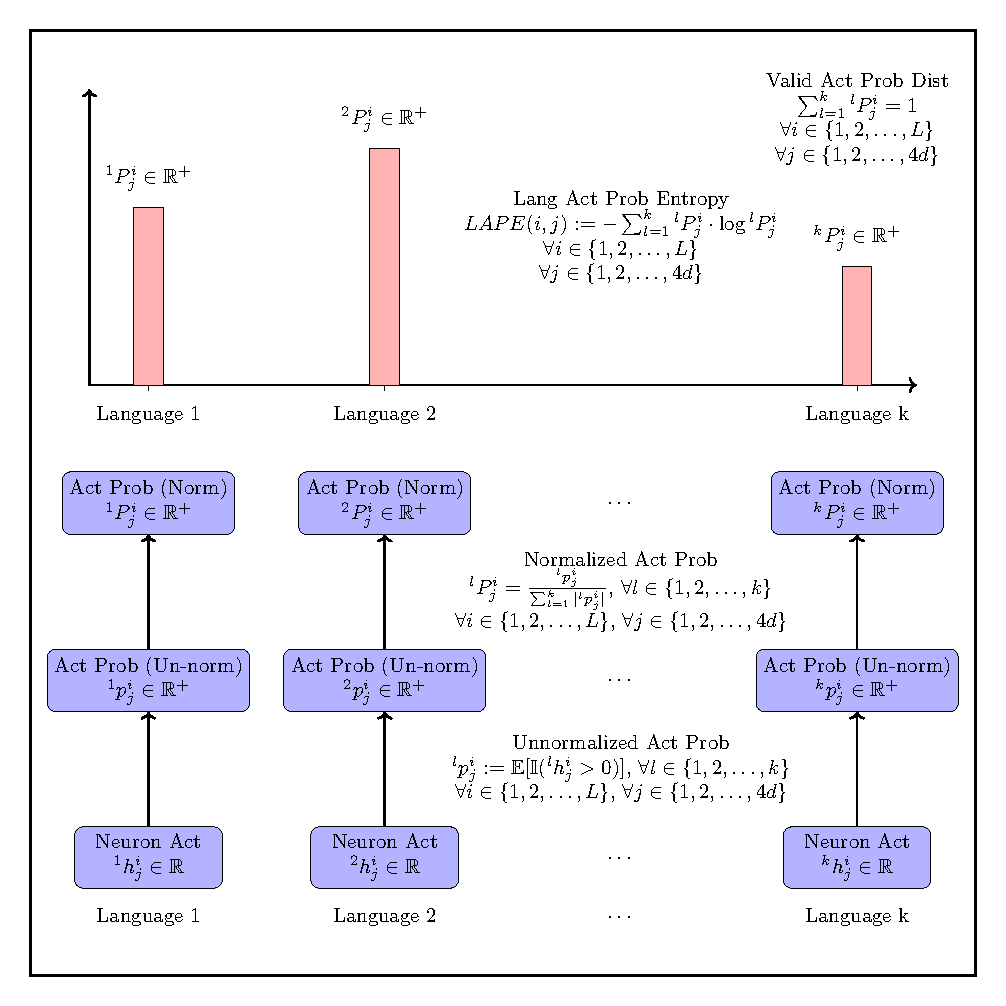
\includegraphics[width=\textwidth]{lape.pdf}
				\end{figure}
			\end{block}
		\end{columns}
	\end{frame}
	
	% ----------------------------------------------------------------------
	% Slide 6: Activation Probability 90p
	% ----------------------------------------------------------------------
	\begin{frame}{Part 1: Language-Specific Neurons}
		\framesubtitle{Methodology: Activation Probability (90p)}
		\begin{columns}
			\column{0.5\textwidth}
			\begin{block}{\scriptsize Relevance from High-Percentile Activations}\scriptsize
				\begin{itemize}
					\item Activation Probability 90p measures how often a neuron's activation exceeds the 90th percentile for its layer, on Wikipedia text.
					\item For neuron $(i,j)$ and language $l$:
					\begin{equation}
						P_q(h_{i,j}^l) = \inf \left\{x \in \mathbb{R} : CDF_{h_{i,j}^l}(x) \geq q \right\},
					\end{equation}
					\begin{equation}
						r_{i,j}^l = \mathbb{E}\left[\mathbb{I}\left(h_{i,j}^l > P_{0.9}(h_{i,j}^l)\right)\right].
					\end{equation}
					\item Relevance values are collected across all neurons:
					\begin{equation}
						R^l = \{r_{i,j}^l \mid i \in \{1, \dots, L\},\ j \in \{1, \dots, 4d\}\}.
					\end{equation}
				\end{itemize}
			\end{block}
			\column{0.4\textwidth}
			\begin{block}{\scriptsize Per-Language Selection}\scriptsize
				\begin{itemize}
					\item For each language, keep the top $0.125\%$ neurons by maximum relevance:
					\begin{equation}
						m = \frac{0.125 \times L \times 4d}{100},
					\end{equation}
					\begin{equation}
						LTN(l) = \text{argsort\_desc}_m \left\{r_{i,j}^l \mid \forall i, j\right\}.
					\end{equation}
					\item This gives the neurons with the highest language-specific relevance for each language.
				\end{itemize}
			\end{block}
		\end{columns}
	\end{frame}
	
	% ----------------------------------------------------------------------
	% Slide 7: Neuron-Targeted LoRA
	% ----------------------------------------------------------------------
	\begin{frame}{Part 1: Language-Specific Neurons}
		\framesubtitle{Methodology: Neuron-Targeted LoRA}
		\begin{columns}
			\column{0.55\textwidth}
			\begin{block}{\scriptsize Freezing Selected Neurons during Fine-Tuning}\scriptsize
				\begin{itemize}
					\item LoRA fine-tunes a low-rank update to the MLP. The masks are
					\begin{equation}
						[\text{masked\_A}]_{ij} = 1, \ \forall i \in \{1,\dots,d\},\ \forall j \in \{1,\dots,r\},
					\end{equation}
					\begin{equation}
						[\text{masked\_B}]_{ij} =
						\begin{cases}
							0, & \text{if } j \in \text{Frozen Neurons}, \\
							1, & \text{otherwise}.
						\end{cases}
					\end{equation}
					\item Zeroing the columns of $B$ at the frozen neurons stops any update to them:
					\begin{equation}
						\Delta W_{i,j} = 0, \quad \forall i \in \{1,\dots,d\},\ \forall j \in \text{Frozen Neurons}.
					\end{equation}
					\item The update applies to the trainable language neurons in the MLP and to the attention projections ($q,k,v,o$).
				\end{itemize}
			\end{block}
			\column{0.35\textwidth}
			\begin{block}{\scriptsize Targeted LoRA Example}\scriptsize
				\begin{figure}
					\centering
					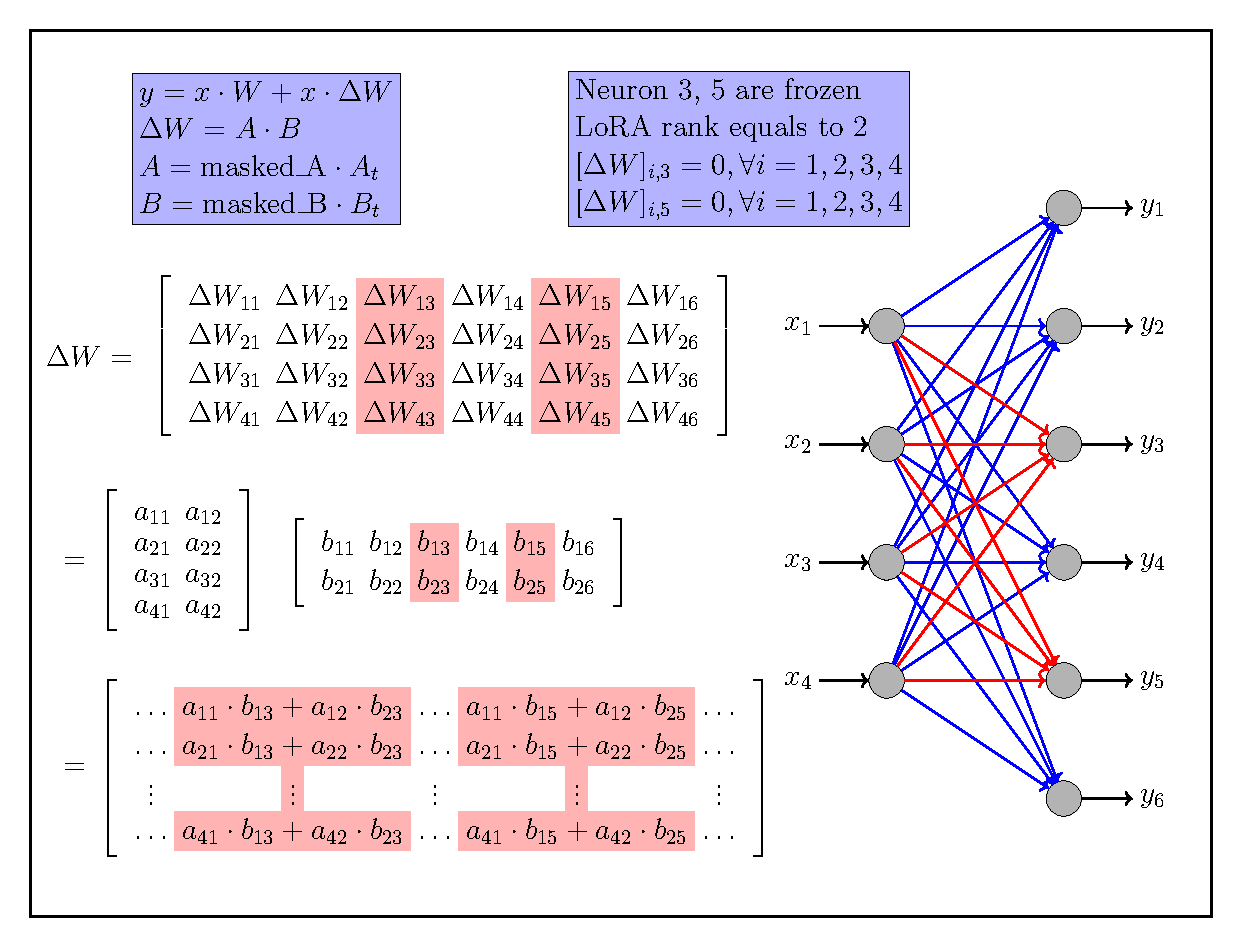
\includegraphics[width=\textwidth]{lora.pdf}
				\end{figure}
			\end{block}
		\end{columns}
	\end{frame}
	
	% ----------------------------------------------------------------------
	% Slide 8: Perplexity Change
	% ----------------------------------------------------------------------
	\begin{frame}{Part 1: Language-Specific Neurons}
		\framesubtitle{Results: Perplexity Change}
		\begin{columns}
			\column{0.55\textwidth}
			\begin{block}{\scriptsize Perplexity Change (PPXC)}\scriptsize
				\begin{itemize}
					\item Checks whether an intervention affects the model's basic handling of a language, before measuring task accuracy.
					\item Defined as the perplexity on language $j$ after intervening on the neurons of language $i$, minus the perplexity with no intervention:
					\begin{equation*}
						\mathrm{PPXC}(i,j) = \mathrm{PPX}\!\left( j \mid \text{intervention on } i \right) - \mathrm{PPX}(j).
					\end{equation*}
					\item A value near zero means little effect; a large value means a strong effect. The diagonal ($i = j$) versus off-diagonal ($i \neq j$) shows whether neurons are language-specific.
				\end{itemize}
			\end{block}
			\column{0.35\textwidth}
			\begin{block}{\scriptsize PPXC Heatmap (Llama 3.1, Zero Int)}\scriptsize
				\begin{figure}[ht]
					\centering
					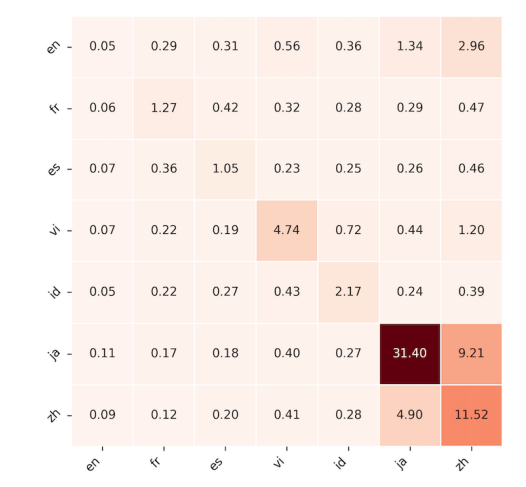
\includegraphics[width=0.9\textwidth]{ppx_fig.png}
				\end{figure}
			\end{block}
		\end{columns}
	\end{frame}
	
	% ----------------------------------------------------------------------
	% Slide 9a: Test-Time Interventions on XNLI
	% ----------------------------------------------------------------------
	\begin{frame}{Part 1: Language-Specific Neurons}
		\framesubtitle{Results: Test-Time Interventions on XNLI}
		\begin{columns}
			\begin{column}{0.35\textwidth}
				\begin{block}{\scriptsize Observations}\scriptsize
					\begin{itemize}
						\item The aim was to improve cross-lingual performance by intervening on language-specific neurons at test time.
						\item Editing the activations does not help and often lowers accuracy, which points to neurons with mixed roles.
					\end{itemize}
				\end{block}
			\end{column}
			\begin{column}{0.55\textwidth}
				\begin{block}{\scriptsize XNLI Accuracy (\%)}\tiny
					\centering
					\setlength{\tabcolsep}{3pt}
					\begin{tabular}{l l c c c c c c c c}
						\toprule
						Model & Lang & No Int & Int $\mu$ & P90 & P95 & Int 0 & P5 & P10 & P25 \\
						\midrule
						Llama 3.1 & vi & 80.5 & 79.5 & 79.0 & 78.9 & 79.8 & 73.6 & 77.7 & 80.5 \\
						(LAPE) & hi & 75.0 & 75.2 & 74.9 & 75.0 & 74.4 & 74.8 & 75.1 & 74.9 \\
						& ur & 70.0 & 70.4 & 69.3 & 69.0 & 68.5 & 68.6 & 68.7 & 69.7 \\
						\midrule
						Llama 3.1 & vi & 80.5 & 78.2 & 79.3 & 79.5 & 79.0 & 76.5 & 77.4 & 78.0 \\
						(Act Prob 90p) & hi & 75.0 & 74.1 & 71.8 & 71.2 & 73.7 & 75.0 & 74.6 & 74.2 \\
						& ur & 70.0 & 69.7 & 69.3 & 68.7 & 69.6 & 69.4 & 69.5 & 69.5 \\
						\midrule
						Mistral Nemo & vi & 80.5 & 80.4 & 80.6 & 80.5 & 79.2 & 80.6 & 80.5 & 80.3 \\
						(LAPE) & hi & 76.1 & 69.8 & 66.9 & 66.6 & 74.9 & 73.0 & 72.4 & 71.0 \\
						& ur & 66.8 & 66.5 & 67.0 & 66.8 & 66.9 & 65.8 & 65.4 & 65.7 \\
						\midrule
						Mistral Nemo & vi & 80.5 & 67.4 & 81.1 & 81.1 & 79.8 & 37.4 & 40.7 & 47.8 \\
						(Act Prob 90p) & hi & 76.1 & 72.2 & 74.5 & 74.4 & 74.5 & 62.4 & 66.3 & 69.3 \\
						& ur & 66.8 & 65.9 & 61.3 & 59.7 & 66.4 & 54.6 & 61.6 & 65.0 \\
						\bottomrule
					\end{tabular}
				\end{block}
			\end{column}
		\end{columns}
	\end{frame}
	
	% ----------------------------------------------------------------------
	% Slide 9b: Test-Time Interventions on XQuAD
	% ----------------------------------------------------------------------
	\begin{frame}{Part 1: Language-Specific Neurons}
		\framesubtitle{Results: Test-Time Interventions on XQuAD}
		\begin{columns}
			\begin{column}{0.15\textwidth}
				\begin{block}{\scriptsize Observations}\scriptsize
					The same edits disrupt task performance on XQuAD, so these neurons take part in task-specific processing and not only language identity.
				\end{block}
			\end{column}
			\begin{column}{0.75\textwidth}
				\begin{block}{\scriptsize XQuAD Results (EM, F1 in parentheses)}\tiny
					\centering
					\setlength{\tabcolsep}{2.5pt}
					\begin{tabular}{l l c c c c c c c c}
						\toprule
						Model & Lang & No Int & Int $\mu$ & P90 & P95 & Int 0 & P5 & P10 & P25 \\
						\midrule
						Llama 3.1 & vi & 41(73.5) & 40(72.9) & 31(69.5) & 28(66.8) & 32(69.2) & 4(35.8) & 10(43.2) & 39(71.5) \\
						(LAPE) & hi & 38(64.1) & 40(65.5) & 36(65.4) & 36(66.3) & 23(49.9) & 38(62.8) & 37(62.8) & 39(65.3) \\
						& zh & 56(77.5) & 10(62.8) & 3(56.1) & 4(52.9) & 33(63.2) & 20(49.1) & 33(63.2) & 22(67.8) \\
						\midrule
						Llama 3.1 & vi & 41(73.6) & 39(73.0) & 23(64.9) & 24(64.8) & 42(73.8) & 33(67.8) & 36(70.3) & 39(72.0) \\
						(Act Prob 90p) & hi & 38(64.1) & 34(60.7) & 36(62.8) & 32(61.9) & 38(62.9) & 23(54.9) & 31(58.6) & 35(60.7) \\
						& zh & 56(77.5) & 61(80.7) & 56(78.8) & 56(78.4) & 55(78.5) & 40(61.7) & 50(73.6) & 56(79.3) \\
						\midrule
						Mistral Nemo & vi & 39(74.6) & 42(76.8) & 40(75.0) & 39(73.6) & 13(45.0) & 10(40.4) & 11(41.2) & 37(73.3) \\
						(LAPE) & hi & 38(66.9) & 35(65.9) & 37(66.6) & 34(66.5) & 22(51.7) & 36(65.8) & 36(66.1) & 36(67.1) \\
						& zh & 47(74.9) & 24(74.0) & 0(61.6) & 0(59.3) & 14(53.3) & 1(33.6) & 24(68.9) & 35(77.0) \\
						\midrule
						Mistral Nemo & vi & 39(74.6) & 11(43.3) & 29(63.9) & 15(48.5) & 39(74.5) & 0(3.8) & 0(6.5) & 2(12.9) \\
						(Act Prob 90p) & hi & 38(66.9) & 26(54.4) & 37(68.9) & 37(68.7) & 33(63.8) & 0(6.0) & 0(11.9) & 12(35.2) \\
						& zh & 47(74.9) & 46(77.4) & 20(59.8) & 15(54.9) & 48(76.2) & 0(8.5) & 0(17.0) & 9(45.6) \\
						\bottomrule
					\end{tabular}
				\end{block}
			\end{column}
		\end{columns}
	\end{frame}
	
	% ----------------------------------------------------------------------
	% Slide 10: Targeted Fine-Tuning
	% ----------------------------------------------------------------------
	\begin{frame}{Part 1: Language-Specific Neurons}
		\framesubtitle{Results: Targeted Fine-Tuning}
		\begin{columns}
			\begin{column}{0.45\textwidth}
				\begin{block}{\scriptsize Observations}\scriptsize
					\begin{itemize}
						\item This tests a longer-lasting intervention: fine-tuning only the language-specific neurons with LoRA.
						\item The result is not distinguishable from standard LoRA fine-tuning.
						\item Both test-time edits and targeted fine-tuning fail to help, which supports moving from internal editing to output-level control.
					\end{itemize}
				\end{block}
			\end{column}
			\begin{column}{0.45\textwidth}
				\begin{block}{\scriptsize Fine-Tuning Results (Llama 3.1)}\tiny
					\centering
					\setlength{\tabcolsep}{4pt}
					\begin{tabular}{l l c c c c c}
						\toprule
						FTL & EL & No Int & Int $\mu$ & P90 & Int 0 & P10 \\
						\midrule
						en & vi & 80.2 & 79.6 & 78.5 & 79.2 & 78.0 \\
						vi & vi & 80.1 & 79.5 & 78.6 & 79.2 & 78.0 \\
						en+vi & vi & 80.1 & 79.4 & 78.5 & 79.1 & 78.0 \\
						\midrule
						en & hi & 74.9 & 74.6 & 74.6 & 74.1 & 74.6 \\
						hi & hi & 74.9 & 74.6 & 74.5 & 74.3 & 74.6 \\
						en+hi & hi & 74.9 & 74.5 & 74.5 & 74.3 & 74.7 \\
						\midrule
						en & ur & 69.8 & 70.4 & 69.6 & 70.2 & 69.0 \\
						ur & ur & 69.8 & 70.5 & 69.5 & 70.4 & 69.1 \\
						en+ur & ur & 70.0 & 70.6 & 69.5 & 70.3 & 68.9 \\
						\bottomrule
					\end{tabular}
				\end{block}
			\end{column}
		\end{columns}
	\end{frame}
	
	% ----------------------------------------------------------------------
	% Slide 11: Findings & Takeaway
	% ----------------------------------------------------------------------
	\begin{frame}{Part 1: Language-Specific Neurons}
		\framesubtitle{Findings and Takeaway}
		\begin{block}{\scriptsize Summary of Findings}\scriptsize
			\begin{itemize}
				\item Direct interventions on language-specific neurons, both at test time and through targeted fine-tuning, do not improve cross-lingual task performance. 
				\item Setting a neuron's activation to zero does not remove its effect, so zero is not a reliable way to turn a neuron off.
				\item The neurons identified for different languages are not independent, so editing the neurons for one language affects the others.
				\item These two observations are consistent with neurons that take part in more than one function \autocite{elhage2022superposition}, which is why surgical edits do not give a clean effect.
			\end{itemize}
		\end{block}
		\begin{alertblock}{\scriptsize Publication accepted at the Sixth Workshop on Insights from Negative Results in NLP, NAACL 2025.}\scriptsize
			\begin{figure}[ht]
				\centering
				
\includegraphics[width=0.9\textwidth]{pub1.png}
			\end{figure}
		\end{alertblock}
	\end{frame}
	
	
	%========================================================================
	%  PART 2 : CROSS-LINGUAL MECHANISMS DURING GRPO TRAINING
	%========================================================================
	
	\partdivider{Part 2}{Cross-Lingual Mechanisms during GRPO Training}
	
	% ----------------------------------------------------------------------
	% Slide: Motivation
	% ----------------------------------------------------------------------
	\begin{frame}{Part 2: Cross-Lingual Mechanisms during GRPO Training}
		\framesubtitle{Motivation}
		\begin{block}{\scriptsize From a Fixed Model to a Training Procedure}\scriptsize
			\begin{itemize}
				\item Part 1 probed a fixed model and found that editing a localized set of neurons does not change task behaviour.
				\item Here we instead track how a training procedure changes a model's cross-lingual behaviour over time.
				\item The procedure is Group Relative Policy Optimization (GRPO) \autocite{shao2024deepseekmath}, used to fine-tune models for reasoning; the behaviour is how the model handles the same math problem in different languages.
			\end{itemize}
		\end{block}
		\begin{block}{\scriptsize Why Reinforcement Learning Raises a Concern}\scriptsize
			\begin{itemize}
				\item GRPO rewards the model only for a correct final answer; the verifier does not read the language of the reasoning.
				\item If the model could raise its reward by leaning more on an English-aligned middle of the stack, training might push it there and widen the gap for low-resource languages.
				\item Whether GRPO actually changes this internal behaviour, and how the effect varies across languages, is the question.
			\end{itemize}
		\end{block}
	\end{frame}
	
	% ----------------------------------------------------------------------
	% Slide: Background -- three-phase hypothesis
	% ----------------------------------------------------------------------
	\begin{frame}{Part 2: Cross-Lingual Mechanisms during GRPO Training}
		\framesubtitle{Background: The Three-Phase Hypothesis}
		\begin{columns}
			\column{0.55\textwidth}
			\begin{block}{\scriptsize Early-Target, Mid-English, Late-Target}\scriptsize
				\begin{itemize}
					\item One account of multilingual transformers \autocite{wendler2024llamas}: early layers map the input into the model's representation; middle layers work in a space closer to English than to the input language; the last layers map back to the input language.
					\item A logit-lens readout of intermediate predictions should then show English through the body of the stack and the target language only near the end.
				\end{itemize}
			\end{block}
			\column{0.45\textwidth}
			\begin{block}{\scriptsize What This Means under GRPO}\scriptsize
				\begin{itemize}
					\item The hypothesis makes a static prediction we can test directly.
					\item Tracking it across checkpoints tests whether GRPO changes it: training could lean more on the English-aligned middle, since the reward ignores the language of the reasoning.
				\end{itemize}
			\end{block}
		\end{columns}
	\end{frame}
	
	% ----------------------------------------------------------------------
	% Slide: Background -- GRPO objective + tools
	% ----------------------------------------------------------------------
	\begin{frame}{Part 2: Cross-Lingual Mechanisms during GRPO Training}
		\framesubtitle{Background: GRPO Objective and Analysis Tools}
		\begin{columns}
			\column{0.52\textwidth}
			\begin{block}{\scriptsize Group Relative Policy Optimization}\scriptsize
				\begin{itemize}
					\item An online policy-gradient method \autocite{shao2024deepseekmath}: for a prompt, the policy generates a group of $G$ responses, each given a scalar reward $R_i^j$.
					\item The advantage standardizes rewards within the group, with no separate value model:
				\end{itemize}
				\begin{equation*}
					A_i^j = \frac{R_i^j - \mu^i}{\sigma^i}, \quad
					\mu^i = \tfrac{1}{G}\sum_{j} R_i^j .
				\end{equation*}
				\begin{itemize}
					\item Loss uses a clipped policy ratio with a KL penalty against a frozen reference ($\epsilon = 0.2$, $\beta = 0.04$).
				\end{itemize}
			\end{block}
			\column{0.48\textwidth}
			\begin{block}{\scriptsize Two Tools for Reading the Model}\scriptsize
				\begin{itemize}
					\item Logit lens \autocite{nostalgebraist2020logitlens}: apply the final normalization and output head to an intermediate layer, giving a per-layer distribution over the vocabulary. We use it to ask which language the predicted token belongs to at each layer.
					\item Centred Kernel Alignment \autocite{kornblith2019similarity}: measures similarity between two sets of representations, invariant to rotation and uniform scaling. We use it to compare a language with English, and a checkpoint with the base model.
				\end{itemize}
			\end{block}
		\end{columns}
	\end{frame}
	
	% ----------------------------------------------------------------------
	% Slide: Experimental setup
	% ----------------------------------------------------------------------
	\begin{frame}{Part 2: Cross-Lingual Mechanisms during GRPO Training}
		\framesubtitle{Experimental Setup}
		\begin{columns}
			\column{0.5\textwidth}
			\begin{block}{\scriptsize Data, Model, and Reward}\scriptsize
				\begin{itemize}
					\item MGSM \autocite{shi2022mgsm}, seven languages: en, bn, te, th, ru, ja, zh. 200 train and 50 eval per language (1{,}400 / 350 total).
					\item One-shot prompts; instruction and field headers in English, question and worked example in the target language; final answer as an English integer.
					\item Policy: Qwen2.5-7B-Instruct ($L=28$, $d=3584$); frozen copy as reference.
					\item Reward is binary, from a verifier combining a regex match with a GPT-4o-mini judge.
				\end{itemize}
			\end{block}
			\column{0.5\textwidth}
			\begin{block}{\scriptsize Training Settings}\scriptsize
				\centering
				\renewcommand{\arraystretch}{1.15}
				\begin{tabular}{ll}
					\toprule
					Setting & Value \\
					\midrule
					LoRA rank $r$ / $\alpha$ & 64 / 16 \\
					LoRA targets & q,k,v,o\_proj \\
					Group size $G$ & 4 \\
					Clip $\epsilon$ / KL $\beta$ & 0.2 / 0.04 \\
					Optimizer & AdamW \\
					Peak LR & $1\times10^{-5}$ \\
					Batch size $B$ & 8 prompts \\
					Total steps & 620 \\
					Checkpoints & every 20 (30 total) \\
					Temperature / $p$ & 0.7 / 0.95 \\
					Max new tokens & 512 \\
					\bottomrule
				\end{tabular}
			\end{block}
		\end{columns}
	\end{frame}
	
	% ----------------------------------------------------------------------
	% Slide: Tokeniser coverage
	% ----------------------------------------------------------------------
	\begin{frame}{Part 2: Cross-Lingual Mechanisms during GRPO Training}
		\framesubtitle{Tokeniser Coverage}
		\begin{columns}
			\column{0.55\textwidth}
			\begin{block}{\scriptsize Script Tokens in the Qwen2.5 Vocabulary}\scriptsize
				\centering
				\renewcommand{\arraystretch}{1.2}
				\begin{tabular}{llc}
					\toprule
					Language & Coverage class & Tokens (approx.) \\
					\midrule
					Chinese  & High (CJK base)  & $\sim 25{,}000$ \\
					Japanese & High (kanji, kana) & $\sim 6{,}000$ \\
					Russian  & High (Cyrillic)  & $\sim 4{,}000$ \\
					Thai     & Mid              & $\sim 2{,}500$ \\
					Bengali  & Low              & $\sim 46$ \\
					Telugu   & Very low         & $\sim 14$ \\
					English  & Bulk of vocab    & --- \\
					\bottomrule
				\end{tabular}
			\end{block}
			\column{0.45\textwidth}
			\begin{block}{\scriptsize What to Note}\scriptsize
				\begin{itemize}
					\item The number of dedicated tokens differs by orders of magnitude across scripts.
					\item Thai has about 2{,}500 tokens, Bengali about 46, Telugu about 14.
					\item This gap lines up with the one language GRPO does not lift, as the results show.
				\end{itemize}
			\end{block}
		\end{columns}
	\end{frame}
	
	% ----------------------------------------------------------------------
	% Slide: The five measurements
	% ----------------------------------------------------------------------
	\begin{frame}{Part 2: Cross-Lingual Mechanisms during GRPO Training}
		\framesubtitle{The Five Measurements}
		\begin{block}{\scriptsize What We Compute at Each Checkpoint}\scriptsize
			\begin{enumerate}
				\item End-task accuracy: fraction of evaluation problems solved per language, judged by the verifier.
				\item Per-layer language distribution: from the logit lens, how much prediction mass falls on each language at each layer, renormalized over the seven languages.
				\item Three-phase analysis: how often the top-1 logit-lens prediction is a given language in the early, middle, and late phases.
				\item English-minus-target gap: per layer, the English fraction minus the target fraction of top-1 predictions.
				\item Representation geometry: CKA cross-lingual similarity to English, and within-language drift from step 0.
			\end{enumerate}
		\end{block}
	\end{frame}
	
	% ----------------------------------------------------------------------
	% Slide: Result 1 -- accuracy
	% ----------------------------------------------------------------------
	\begin{frame}{Part 2: Cross-Lingual Mechanisms during GRPO Training}
		\framesubtitle{Result: Accuracy over Training}
		\begin{columns}
			\column{0.58\textwidth}
			\begin{block}{\scriptsize Accuracy across 620 Steps}\scriptsize
				\centering
				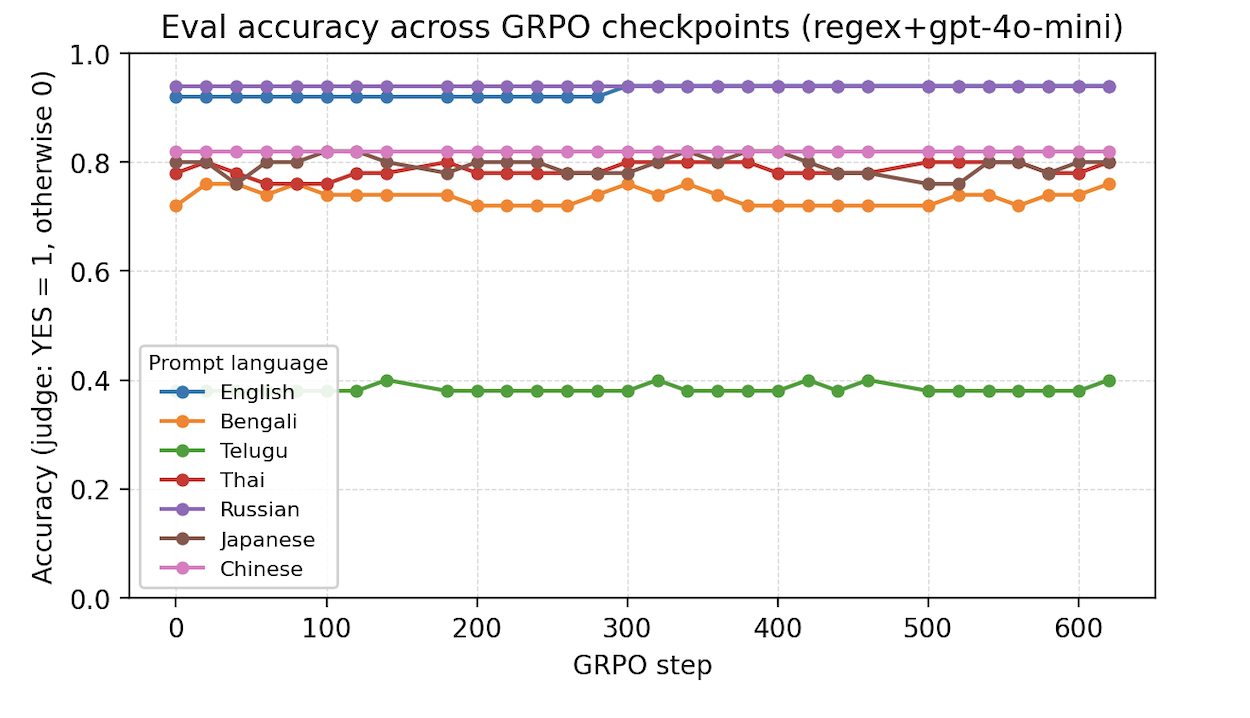
\includegraphics[width=\linewidth]{accuracy_gpt.png}
			\end{block}
			\column{0.42\textwidth}
			\begin{block}{\scriptsize First and Last Checkpoint}\scriptsize
				\centering
				\renewcommand{\arraystretch}{1.15}
				\begin{tabular}{lccc}
					\toprule
					Lang & Step 0 & Step 620 & $\Delta$ \\
					\midrule
					en & 0.92 & 0.94 & $+0.02$ \\
					ru & 0.94 & 0.94 & $+0.00$ \\
					zh & 0.82 & 0.82 & $+0.00$ \\
					ja & 0.80 & 0.80 & $+0.00$ \\
					th & 0.78 & 0.80 & $+0.02$ \\
					bn & 0.72 & 0.76 & $+0.04$ \\
					te & 0.38 & 0.40 & $+0.02$ \\
					\bottomrule
				\end{tabular}
				\vspace{0.4em}
				\begin{itemize}
					\item Six languages stay between about 0.72 and 0.94; Telugu stays at about 0.38 to 0.40.
					\item GRPO moves accuracy by at most a few points.
				\end{itemize}
			\end{block}
		\end{columns}
	\end{frame}
	
	% ----------------------------------------------------------------------
	% Slide: Result 2 -- per-layer language
	% ----------------------------------------------------------------------
	\begin{frame}{Part 2: Cross-Lingual Mechanisms during GRPO Training}
		\framesubtitle{Result: Predicted Language at Each Layer}
		\begin{columns}
			\column{0.6\textwidth}
			\begin{block}{\scriptsize Logit-Lens Language by Layer and Step}\scriptsize
				\centering
				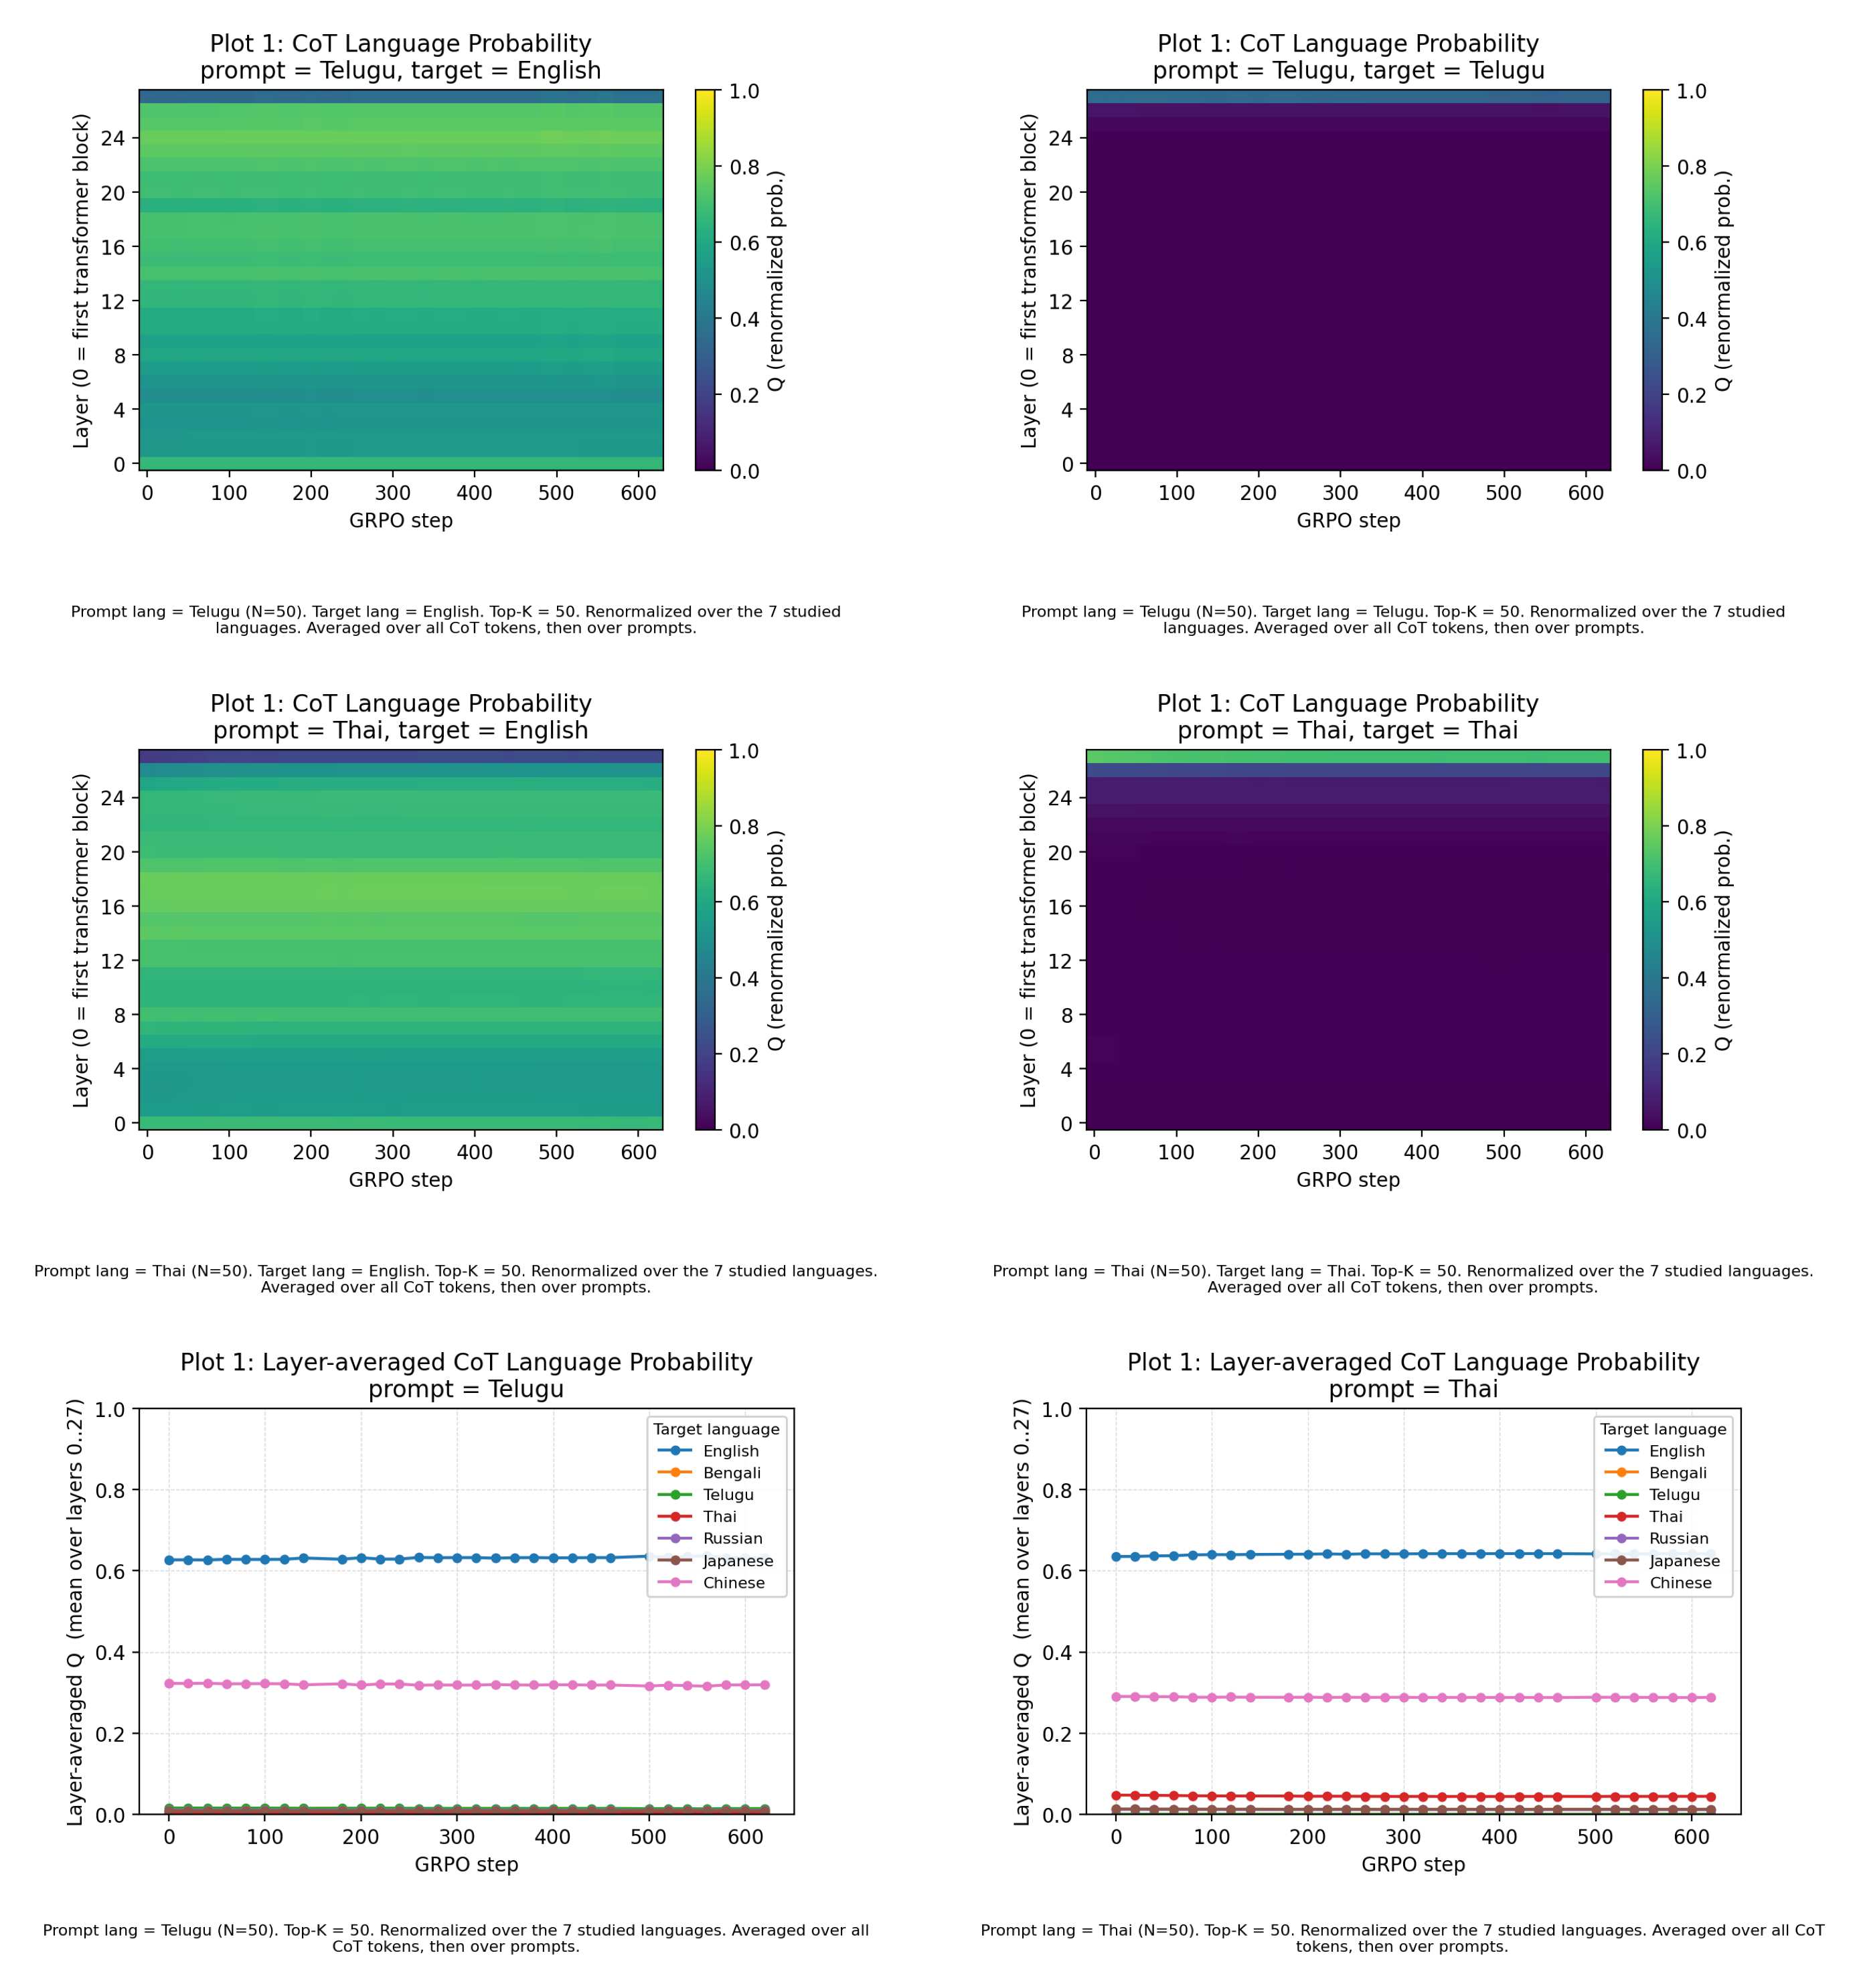
\includegraphics[width=\linewidth]{combined_plot1.png}
			\end{block}
			\column{0.4\textwidth}
			\begin{block}{\scriptsize Reading}\scriptsize
				\begin{itemize}
					\item For a non-English prompt, early and middle layers put most mass on English; the target language appears only in the last two or three layers.
					\item The pattern is the same across prompt languages.
					\item It is flat across all 620 steps: GRPO neither builds up nor removes the English-leaning middle.
				\end{itemize}
			\end{block}
		\end{columns}
	\end{frame}
	
	% ----------------------------------------------------------------------
	% Slide: Result 3 -- three-phase and gap
	% ----------------------------------------------------------------------
	\begin{frame}{Part 2: Cross-Lingual Mechanisms during GRPO Training}
		\framesubtitle{Result 3: Three-Phase Analysis and the English Lead}
		\begin{block}{\scriptsize Top-1 Language per Phase and the English-Minus-Target Gap}\scriptsize
			\centering
			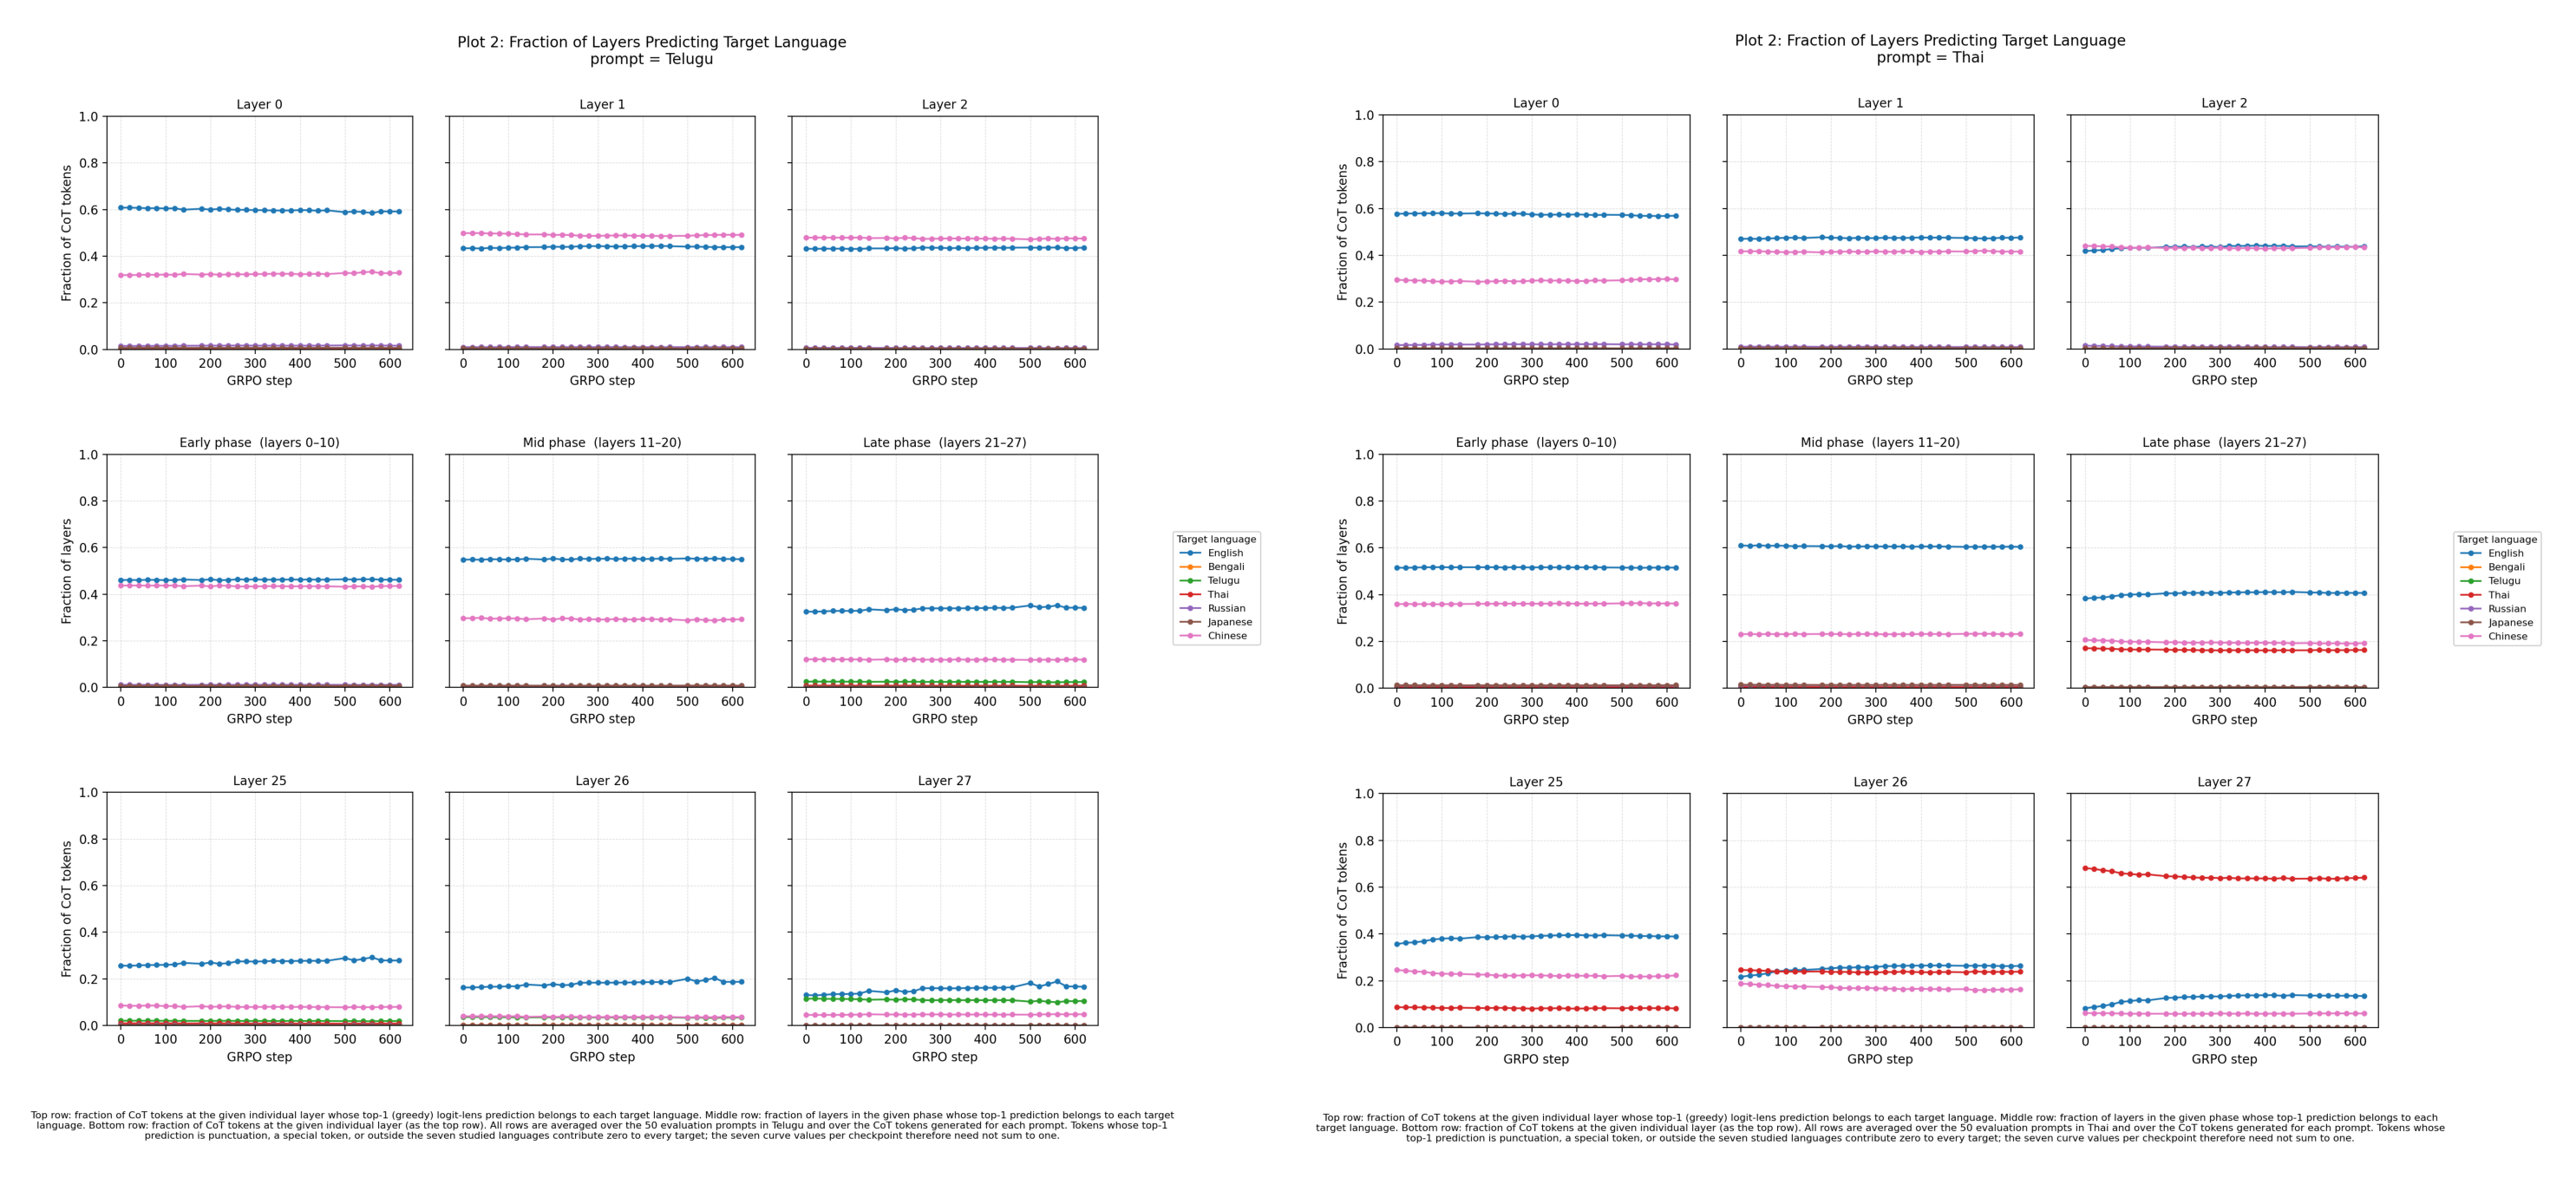
\includegraphics[width=0.48\linewidth]{combined_plot2.png}\hfill
			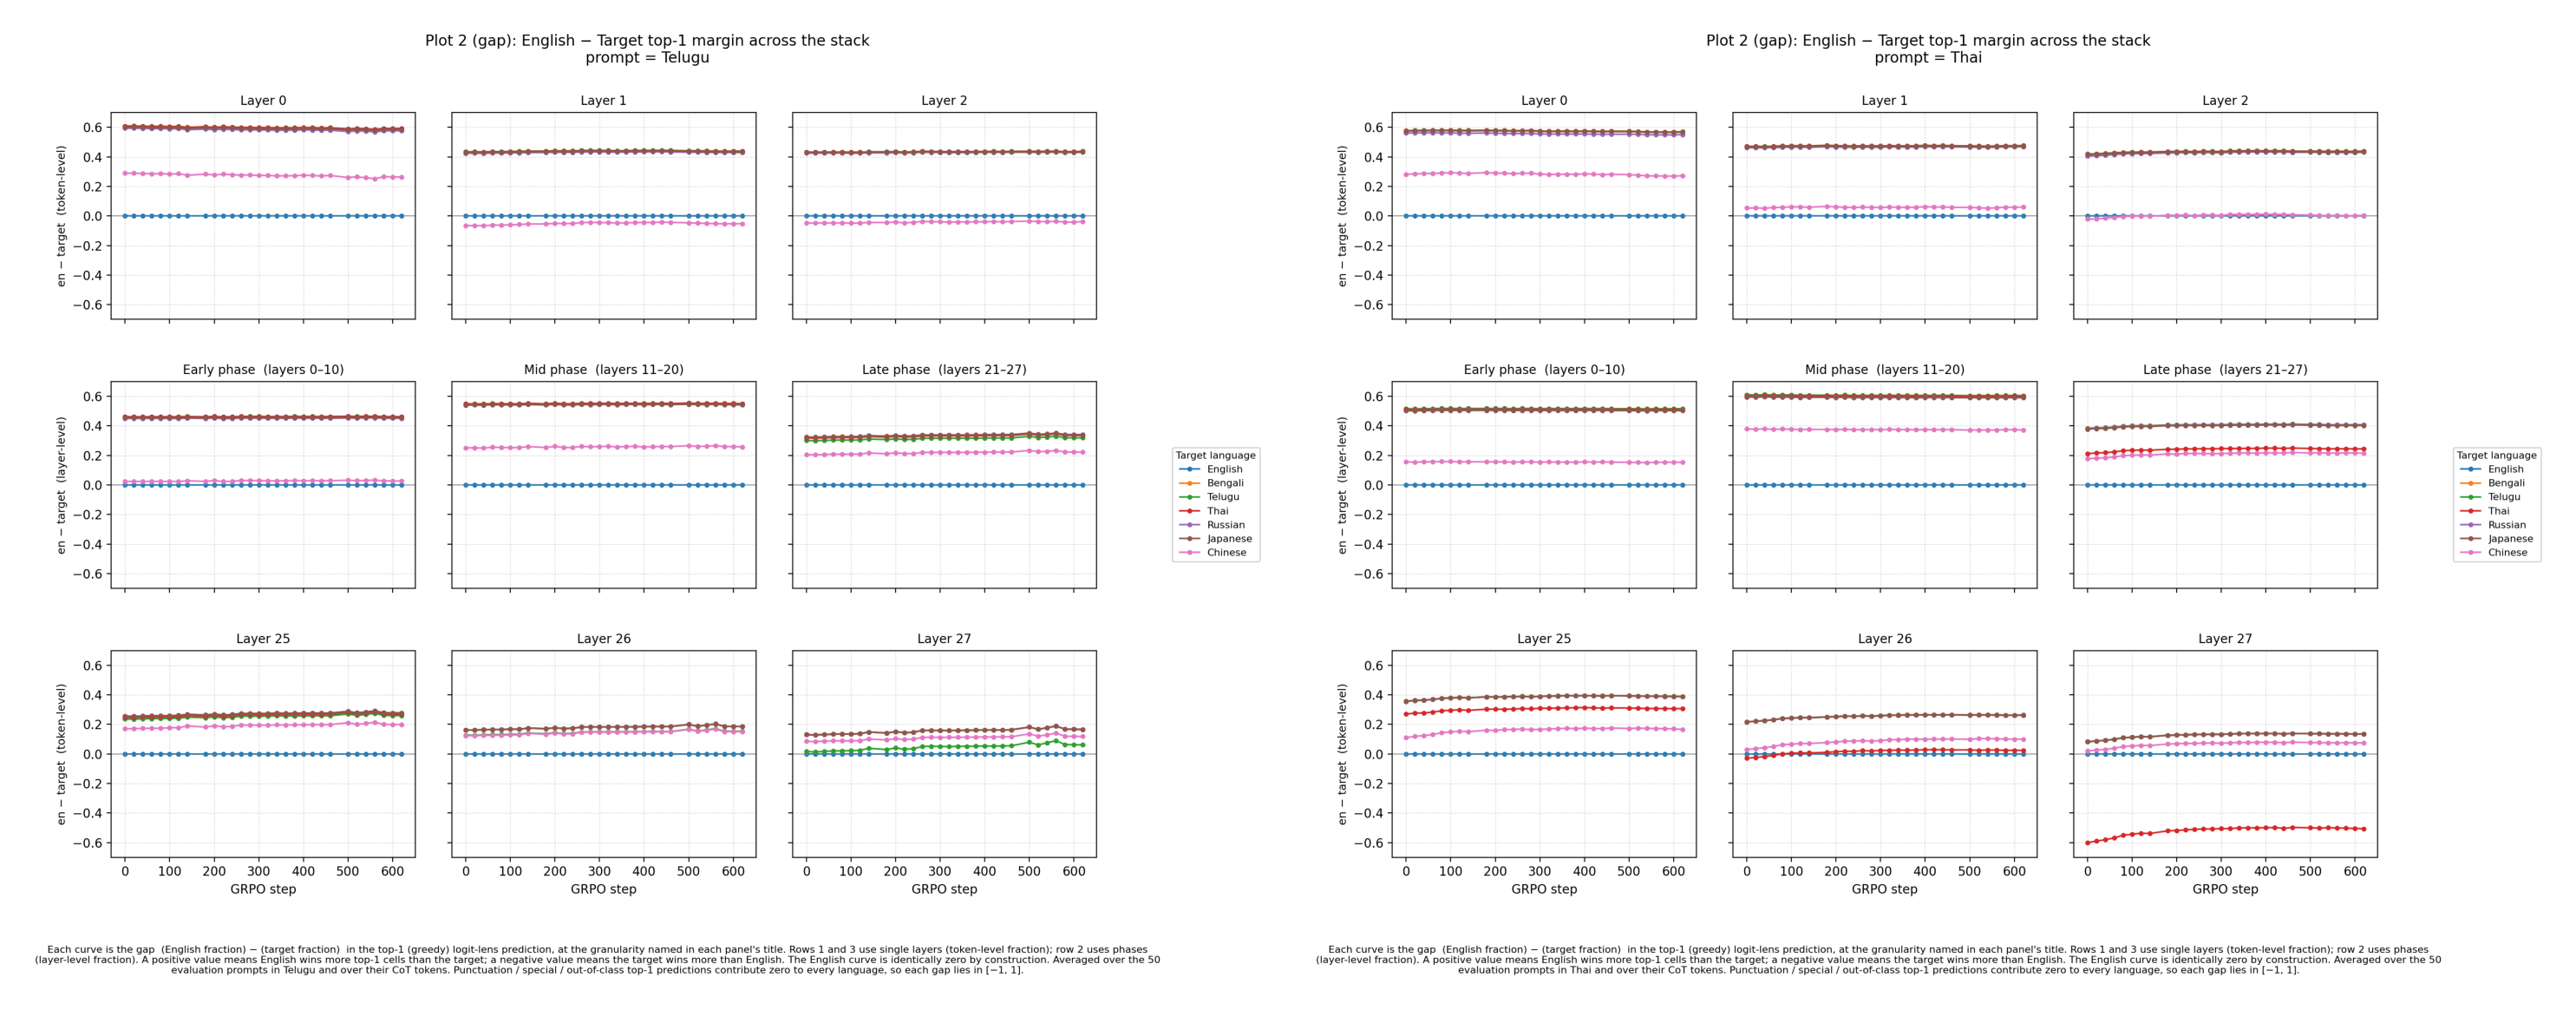
\includegraphics[width=0.48\linewidth]{combined_plot2_gap.png}
		\end{block}
		\begin{block}{\scriptsize Reading}\scriptsize
			\begin{itemize}
				\item English leads the early and middle phases, highest in the middle; the target language appears mainly in the late phase.
				\item At the last layer, Thai overtakes English while Telugu stays low. The English-minus-target gap is positive through the body of the stack and flat across the 620 steps.
			\end{itemize}
		\end{block}
	\end{frame}
	
	% ----------------------------------------------------------------------
	% Slide: Result 4 -- CKA
	% ----------------------------------------------------------------------
	\begin{frame}{Part 2: Cross-Lingual Mechanisms during GRPO Training}
		\framesubtitle{Result: Representation Geometry (CKA)}
		\begin{columns}
			\column{0.58\textwidth}
			\begin{block}{\scriptsize Cross-Lingual Similarity and Within-Language Drift}\scriptsize
				\centering
				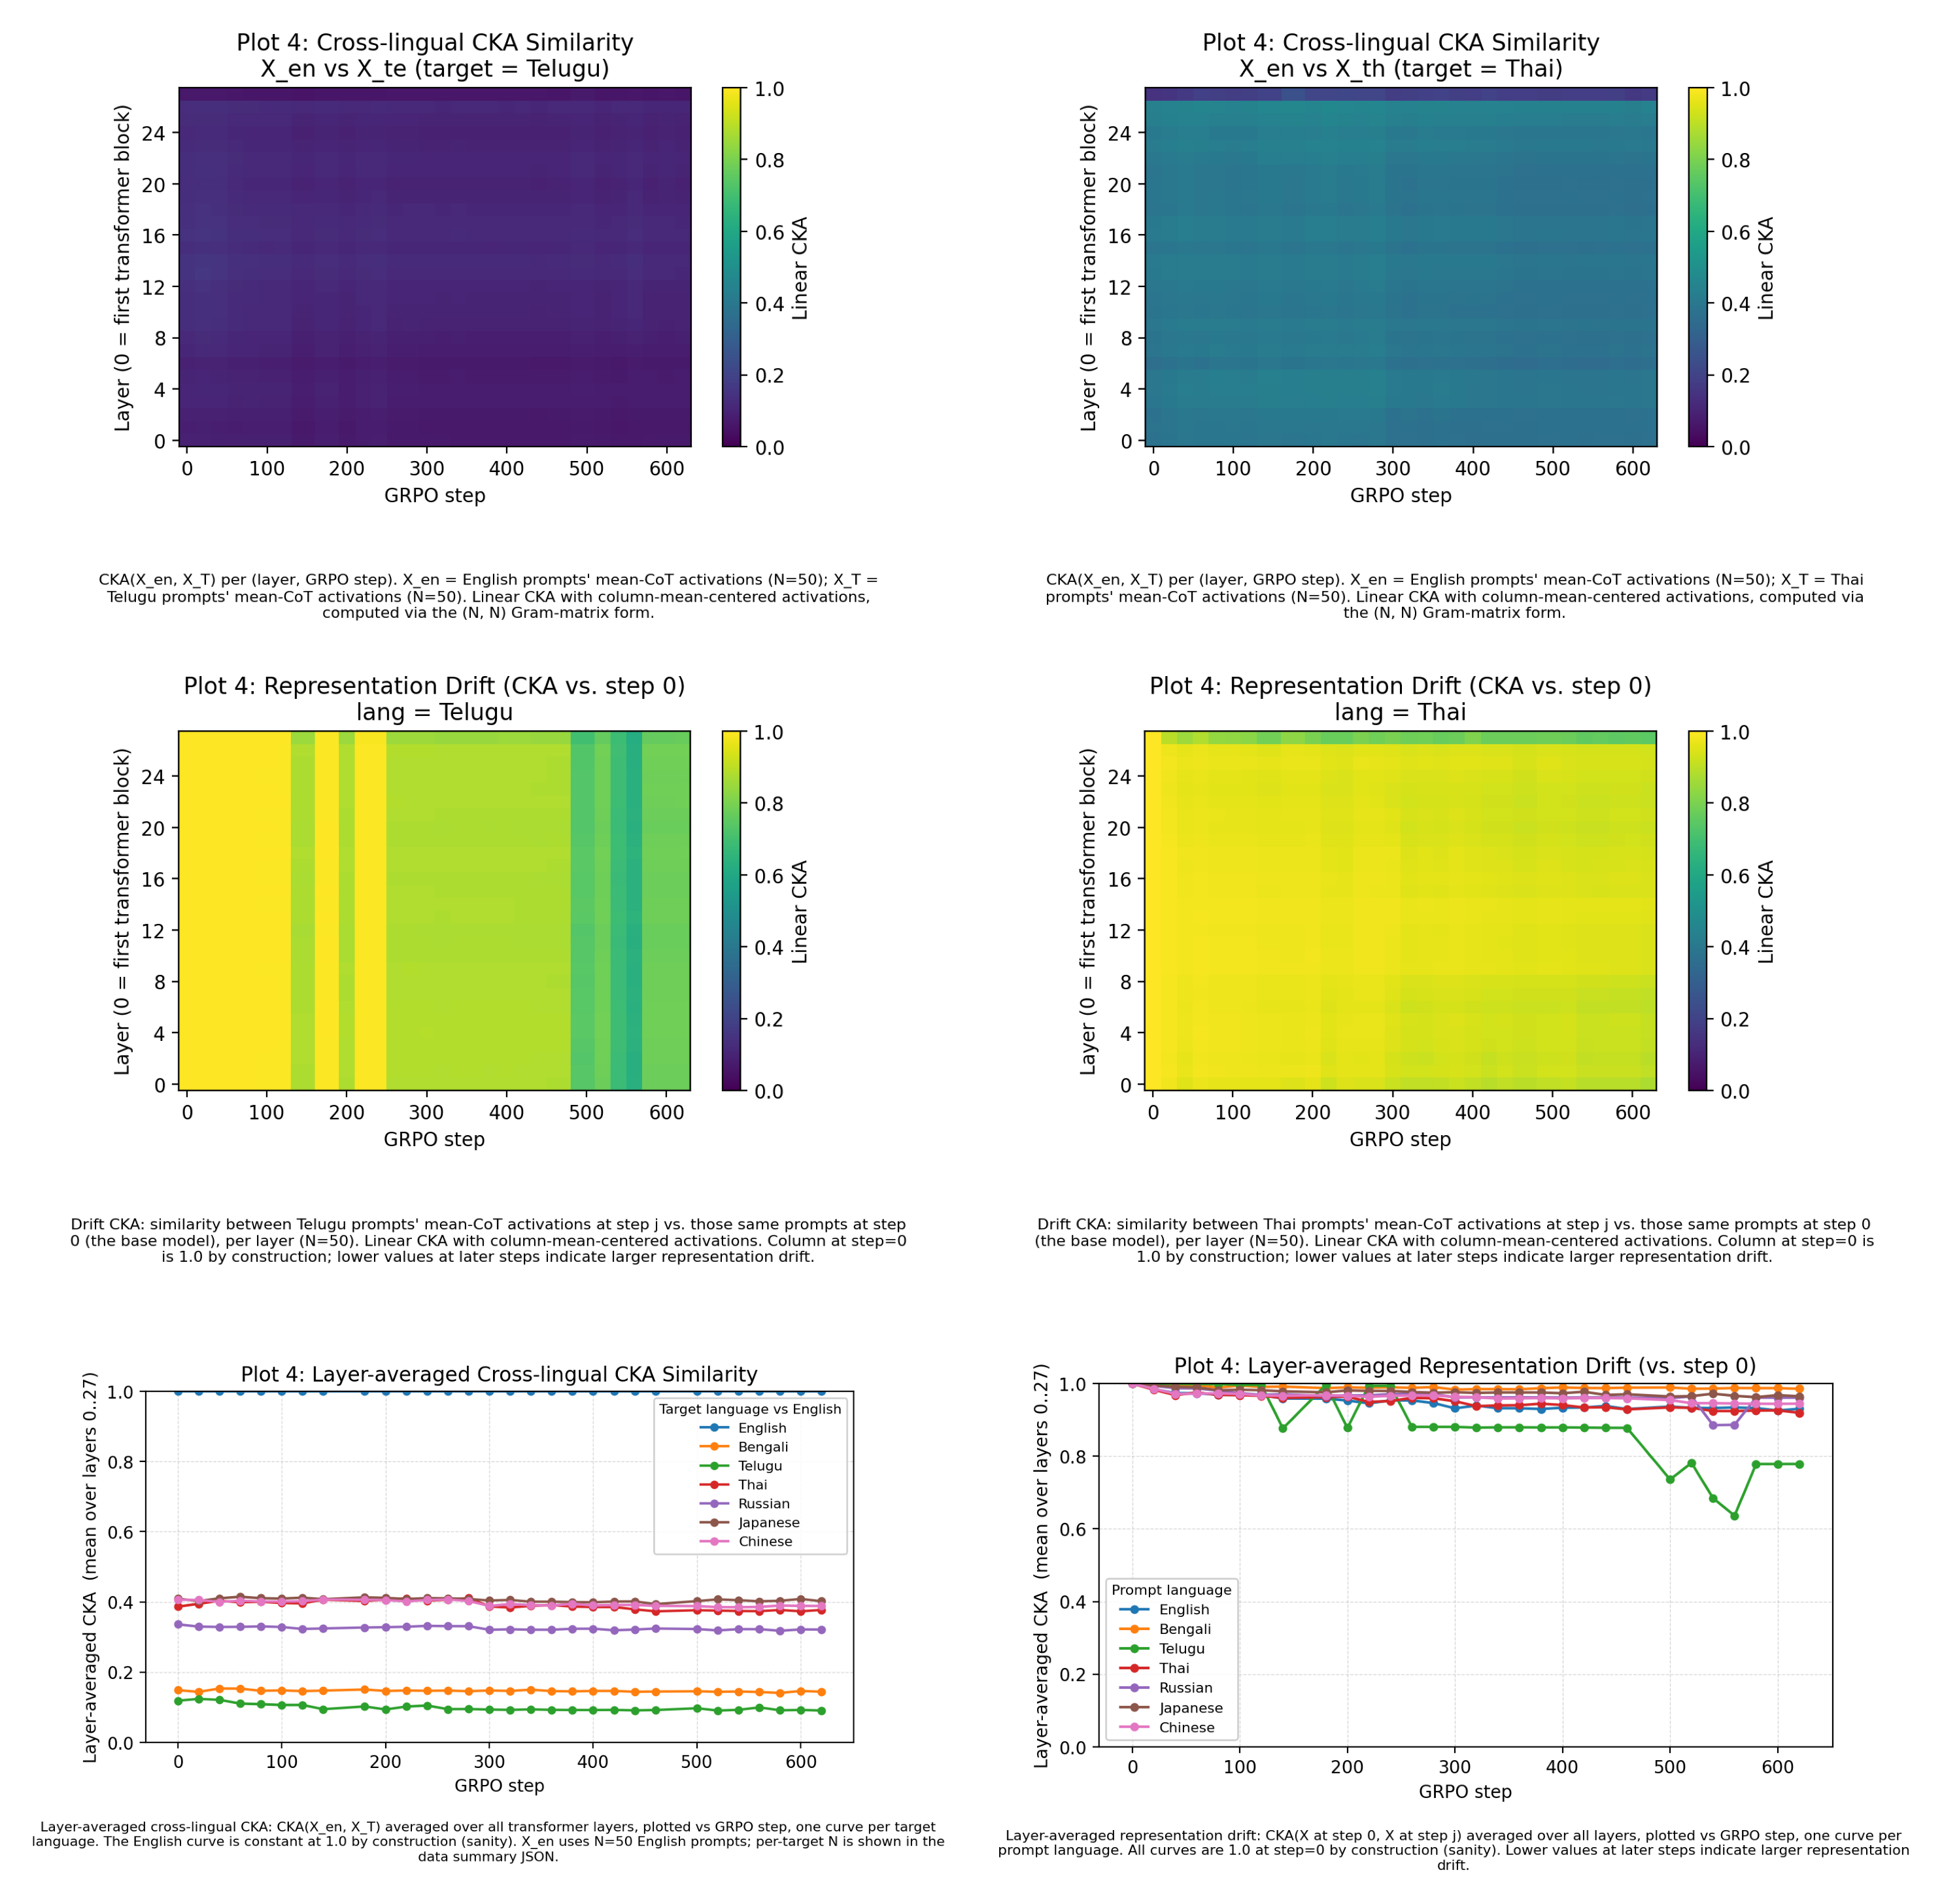
\includegraphics[width=\linewidth]{combined_plot4.png}
			\end{block}
			\column{0.42\textwidth}
			\begin{block}{\scriptsize Reading}\scriptsize
				\begin{itemize}
					\item Similarity to English is flat over training and tracks coverage: Telugu and Bengali lowest (about 0.10 and 0.15), Russian about 0.32, Thai/Japanese/Chinese about 0.40.
					\item Within-language drift: every language stays above about 0.90, except Telugu, which drops to about 0.63 before settling near 0.78.
					\item The one language that does not improve is the one whose representations move the most.
				\end{itemize}
			\end{block}
		\end{columns}
	\end{frame}
	
	% ----------------------------------------------------------------------
	% Slide: Discussion
	% ----------------------------------------------------------------------
	\begin{frame}{Part 2: Cross-Lingual Mechanisms during GRPO Training}
		\framesubtitle{Discussion}
		\begin{block}{\scriptsize GRPO Does Not Cause Cross-Lingual Collapse}\scriptsize
			\begin{itemize}
				\item The model reads out as English through the early and middle layers and surfaces the target language only at the end, matching the static three-phase picture.
				\item This is already present at step 0 and does not change over 620 steps. The per-layer distribution, the three-phase commitment, and the English-minus-target gap are all flat in training.
			\end{itemize}
		\end{block}
		\begin{block}{\scriptsize Tokeniser Coverage and the Telugu Case}\scriptsize
			\begin{itemize}
				\item Telugu sits far below the rest, does not improve, and is also the language whose representations move the most.
				\item With very few dedicated tokens, its text is split into long, coarse byte sequences, so the answer-level reward does not turn into a useful per-token gradient.
				\item The limiting factor is the granularity of the reward signal, set by coverage, not language identity or a change in internal routing.
			\end{itemize}
		\end{block}
	\end{frame}
	
	
	
	
	
	%========================================================================
	%  PART 3 : FairPO
	%========================================================================
	
	\partdivider{Part 3}{FairPO: Robust Preference Optimization for Fair Multi-Label Learning}
	
	% ----------------------------------------------------------------------
	% Slide 23: Motivation
	% ----------------------------------------------------------------------
	\begin{frame}{Part 3: FairPO}
		\framesubtitle{Motivation: Fair Multi-Label Learning}
		\begin{block}{\scriptsize Where Standard Training Falls Short}\scriptsize
			Multi-label classification (MLC) is used in content tagging, medical diagnosis support, and skill identification from resumes. Models trained to optimize overall metrics can:
			\begin{itemize}
				\item Do well on frequent labels (non-privileged, $\nonprivileged$) but poorly on rare but important labels (privileged, $\privileged$).
				\item Leave a large gap between the two groups: $perf(\privileged) \ll perf(\nonprivileged)$.
				\item Example: a medical system that keeps missing rare disease labels in $\privileged$.
			\end{itemize}
			Standard losses such as BCE do not account for this, and simple re-weighting does not reliably balance the two groups or handle confusing labels.
		\end{block}
		\begin{block}{\scriptsize What FairPO Aims to Do}\scriptsize
			\begin{itemize}
				\item Target the performance gap between the two label groups $\privileged$ and $\nonprivileged$ directly.
				\item Use robust optimization to balance the groups, so improving one does not come at the cost of the other.
			\end{itemize}
		\end{block}
	\end{frame}
	
	% ----------------------------------------------------------------------
	% Slide 24: Problem Setup & Fairness Goals
	% ----------------------------------------------------------------------
	\begin{frame}{Part 3: FairPO}
		\framesubtitle{Problem Setup and Fairness Goals}
		\begin{block}{\scriptsize Setup, Confusing Sets, and the Two Goals}\scriptsize
			\begin{itemize}
				\item MLC with $T$ labels, $\labels = \{1,\dots,T\}$, dataset $\dataset = \{(x_i, y_i)\}_{i=1}^N$, with $y_{il} = +1$ if label $l$ applies to $x_i$ and $0$ otherwise.
				\item Partition $\labels$ into privileged $\privileged$ and non-privileged $\nonprivileged$. Model score for label $t$ is $\model(x_i; \params_t)$; reference score is $\model(x_i; \refparams_t)$.
				\item Confusing sets for a privileged label $l \in \privileged$:
				\begin{itemize}\scriptsize
					\item If $y_{il} = +1$: confusing negatives $S_{il}^{\text{neg}} = \{ k \mid y_{ik} = 0,\ \model(x_i; \params_k) \ge \model(x_i; \params_l) \}$.
					\item If $y_{il} = 0$: confusing positives $S_{il}^{\text{pos}} = \{ k' \mid y_{ik'} = +1,\ \model(x_i; \params_{k'}) \le \model(x_i; \params_l) \}$.
				\end{itemize}
				Overall confusing set $S_{il} = S_{il}^{\text{neg}} \cup S_{il}^{\text{pos}}$.
				\item Fairness goals:
				\begin{itemize}\scriptsize
					\item Privileged: if $S_{il} \neq \emptyset$, push $\model(x_i; \params_l) \gg \model(x_i; \params_k)$ for $k \in S_{il}^{\text{neg}}$ and $\model(x_i; \params_l) \ll \model(x_i; \params_{k'})$ for $k' \in S_{il}^{\text{pos}}$; otherwise use BCE.
					\item Non-privileged: keep performance close to the reference, $\baseloss(\params_j) \le \baseloss(\refparams_j) + \epsilon$.
				\end{itemize}
			\end{itemize}
		\end{block}
	\end{frame}
	
	% ----------------------------------------------------------------------
	% Slide 25: Preference-Based Privileged Loss
	% ----------------------------------------------------------------------
	\begin{frame}{Part 3: FairPO}
		\framesubtitle{Preference-Based Privileged Loss}
		\begin{block}{\scriptsize Framing Hard Privileged Cases as Preferences}\scriptsize
			\begin{itemize}
				\item For a privileged label $l$ that is truly positive, the model may score a confusing negative $k \in S_{il}^{\text{neg}}$ higher; we want $\model(x_i; \params_l) \gg \model(x_i; \params_k)$.
				\item For a privileged label $l$ that is truly negative, the model may score it above an actual positive $k' \in S_{il}^{\text{pos}}$; we want $\model(x_i; \params_l) \ll \model(x_i; \params_{k'})$.
				\item Following DPO \autocite{rafailov2023direct}, we treat these as preferences ($l \succ k$, or $l \prec k'$ in score terms) and use a comparison term measured against a reference. If $S_{il} = \emptyset$, BCE is used for label $l$.
			\end{itemize}
		\end{block}
		\begin{block}{\scriptsize Privileged Loss}\scriptsize
			\begin{equation}
				h_{\params}(x_i, l, k) = \left( \log \frac{\model(x_i; \params_l)}{\model(x_i; \refparams_l)} \right) - \left( \log \frac{\model(x_i; \params_k)}{\model(x_i; \refparams_k)} \right).
			\end{equation}
			\begin{equation}
				\loss_{\privileged} = \E_{(x_i, l, k)\,:\, l \in \privileged,\, y_{il}=+1,\, k \in \confusing} \left[ -\log \sigma \left( \beta \cdot h_{\params}(x_i, l, k) \right) \right].
			\end{equation}
			Minimizing $\loss_{\privileged}$ makes $h_{\params}$ large and positive, so the model separates true positive privileged labels from their confusing negatives, relative to the reference.
		\end{block}
	\end{frame}
	
	% ----------------------------------------------------------------------
	% Slide 26: Constrained Non-Privileged Loss
	% ----------------------------------------------------------------------
	\begin{frame}{Part 3: FairPO}
		\framesubtitle{Constrained Non-Privileged Loss}
		\begin{block}{\scriptsize Keeping Non-Privileged Performance Near the Reference}\scriptsize
			\begin{itemize}
				\item For non-privileged labels $j \in \nonprivileged$, the goal is to keep performance from dropping relative to the reference $\refparams_j$ while the model focuses on privileged labels.
				\item Base BCE loss for label $j$ and instance $x_i$:
				\begin{align}
					loss(\params_j) &= -y_{ij} \log \model(x_i;\params_j) - (1-y_{ij})\log (1-\model(x_i;\params_j)), \\
					loss(\refparams_j) &= -y_{ij} \log \model(x_i;\refparams_j) - (1-y_{ij})\log (1-\model(x_i;\refparams_j)).
				\end{align}
				\item A hinge penalizes the model only when the increase in loss over the reference exceeds a slack $\epsilon \ge 0$:
				\begin{align}
					\loss_{\nonprivileged} &= \E_{(x_i,\, \{y_{ij}\,:\, j \in \nonprivileged\})} \left[ L_h(\params_j, \refparams_j; \epsilon) \right], \\
					L_h(\params_j, \refparams_j; \epsilon) &= \max \left( 0,\ loss(\params_j) - loss(\refparams_j) - \epsilon \right).
				\end{align}
			\end{itemize}
		\end{block}
	\end{frame}
	
	% ----------------------------------------------------------------------
	% Slide 27: Group-Robust Balancing & Algorithm
	% ----------------------------------------------------------------------
	\begin{frame}{Part 3: FairPO}
		\framesubtitle{Group-Robust Balancing and Algorithm}
		\begin{columns}
			\column{0.52\textwidth}
			\begin{block}{\scriptsize Balancing the Two Group Losses}\scriptsize
				\begin{itemize}
					\item The two losses pull against each other, and a fixed weighted sum does not adapt during training.
					\item We treat the two label groups as the groups in Group Robust Preference Optimization (GRPO = Group Robust Preference Optimization) \autocite{ramesh2024group} and write a minimax objective:
				\end{itemize}
				\begin{equation}
					\min_{\{\params_t\}} \max_{\alpha \in \Delta} \left[ \alpha_{\privileged} \loss_{\privileged} + \alpha_{\nonprivileged} \loss_{\nonprivileged} \right].
				\end{equation}
				\begin{itemize}
					\item The weights $\alpha = (\alpha_{\privileged}, \alpha_{\nonprivileged})$ live on the simplex $\Delta$. The inner step puts more weight on whichever group currently has the higher loss; the outer step updates the model under that weighting.
				\end{itemize}
			\end{block}
			\column{0.48\textwidth}
			\begin{block}{\scriptsize Training Procedure}\scriptsize
				\begin{itemize}
					\item Solved by alternating mirror ascent on $\alpha$ and mirror descent on $\params$.
					\item For stability, $\alpha$ is updated from each group's loss relative to its running average, since the two losses can be on different scales.
				\end{itemize}
				\begin{figure}
					\centering
					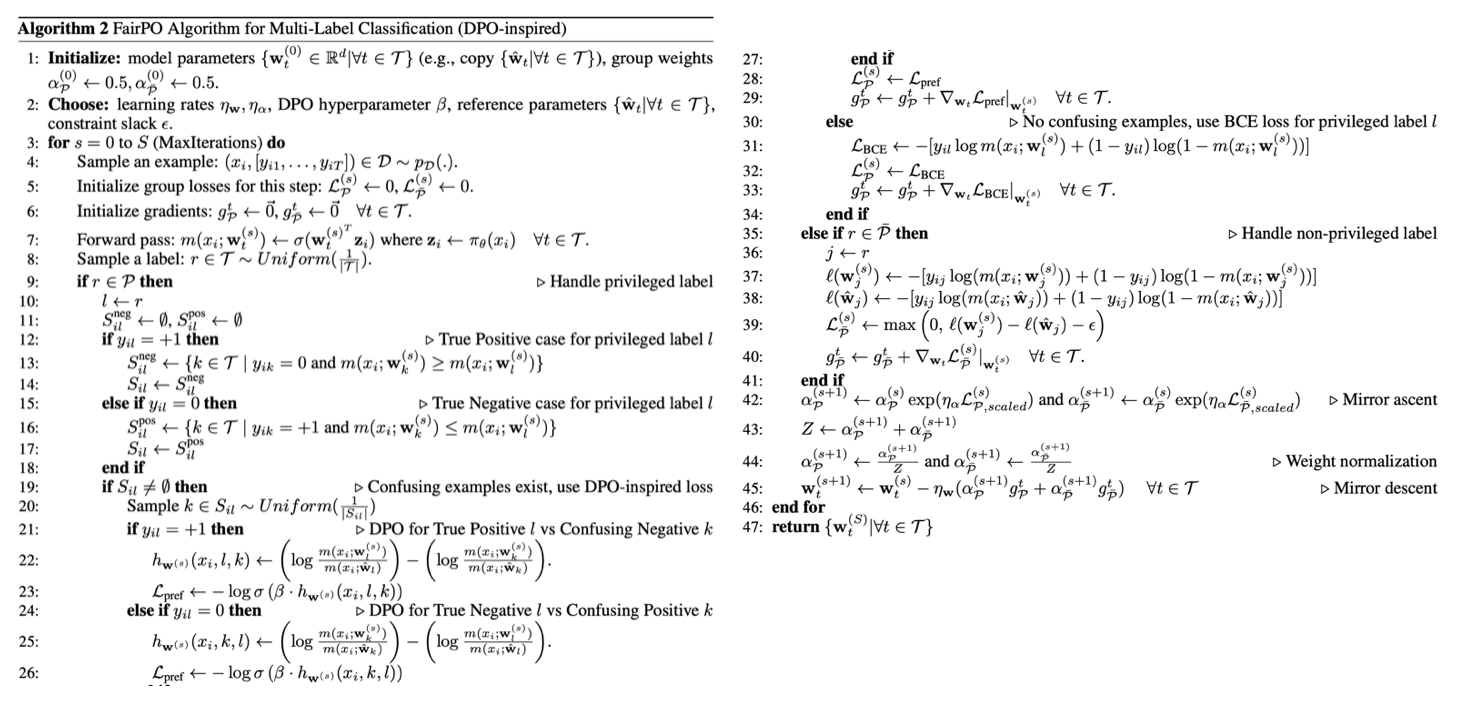
\includegraphics[width=\textwidth]{fairpo-algo-full.png}
				\end{figure}
			\end{block}
		\end{columns}
	\end{frame}
	
	% ----------------------------------------------------------------------
	% Slide 28: SimPO / CPO Variants
	% ----------------------------------------------------------------------
	\begin{frame}{Part 3: FairPO}
		\framesubtitle{SimPO and CPO Variants}
		\begin{block}{\scriptsize SimPO-Based Privileged Loss}\scriptsize
			SimPO \autocite{meng2024simpo} is reference-free and adds a target margin $\gamma$. Applied here, it compares the model's confidence on the true positive label $l$ against the confusing negative $k$:
			\begin{equation}
				\loss_{\privileged}^{\text{SimPO}} = \E_{(x_i, l, k)\,:\, l \in \privileged,\, y_{il}=+1,\, k \in \confusing} \left[ -\log \sigma \left( \beta \left( \log \frac{m(x_i;\params_l)}{m(x_i;\params_k)} \right) - \gamma \right) \right].
			\end{equation}
		\end{block}
		\begin{block}{\scriptsize CPO-Based Privileged Loss}\scriptsize
			CPO \autocite{xu2024contrastive} combines a margin-free preference term with an NLL regularizer on the true positive privileged label:
			\begin{equation}
				L_{\mathcal{P}}^{\text{CPO-prefer}} = \E_{(x_i, l, k)} \left[ -\log \sigma \left( \beta \log \frac{m(x_i;\params_l)}{m(x_i;\params_k)} \right) \right], \quad
				L_{\mathcal{P}}^{\text{CPO-NLL}} = \E_{(x_i, l)} [ -\log \model(x_i; \params_l) ].
			\end{equation}
			\begin{equation}
				\loss_{\privileged}^{\text{CPO}} = L_{\mathcal{P}}^{\text{CPO-prefer}} + \lambda\, L_{\mathcal{P}}^{\text{CPO-NLL}}.
			\end{equation}
			Each variant replaces only the preference term inside the privileged loss; the balancing and non-privileged handling stay the same.
		\end{block}
	\end{frame}
	
	% ----------------------------------------------------------------------
	% Slide 29: Results on MS-COCO and NUS-WIDE
	% ----------------------------------------------------------------------
	\begin{frame}{Part 3: FairPO}
		\framesubtitle{Results: MS-COCO and NUS-WIDE}
		\begin{block}{\scriptsize MS-COCO ($\privileged$ = 20\% least frequent labels, $\nonprivileged$ = remaining 80\%)}\scriptsize
			\centering
			\tiny
			\adjustbox{max width=\textwidth}{%
				\begin{tabular}{lcccccccccc}
					\toprule
					\multicolumn{1}{c}{Method} & \multicolumn{2}{c}{mAP} & \multicolumn{2}{c}{Sample F1} & \multicolumn{2}{c}{Accuracy} & \multicolumn{2}{c}{EMR} & \multicolumn{1}{c}{$\Delta \text{mAP}(\mathcal{P})$} \\
					\cmidrule(lr){2-3} \cmidrule(lr){4-5} \cmidrule(lr){6-7} \cmidrule(lr){8-9}
					& $\mathcal{P}$ & $\nonprivileged$ & $\mathcal{P}$ & $\nonprivileged$ & $\mathcal{P}$ & $\nonprivileged$ & $\mathcal{P}$ & $\nonprivileged$ & \\
					\midrule
					BCE SFT      & 86.32 & 90.65 & 61.43 & 64.89 & 94.89 & 98.12 & 35.78 & 36.98 & Ref \\
					BCE SFT + RW & 87.25 & 89.85 & 62.68 & 64.11 & 95.95 & 97.93 & 47.43 & 33.81 & +0.93 \\
					GDRO + BCE   & 87.92 & 90.41 & 62.31 & 64.75 & 95.72 & 98.05 & 46.12 & 35.16 & +1.60 \\
					\midrule
					FairPO-DPO   & 88.02 & 89.97 & 63.45 & 63.65 & 97.89 & 98.04 & 62.19 & 35.12 & +1.70 \\
					FairPO-SimPO & 87.67 & 88.76 & 62.34 & 63.12 & 95.69 & 97.78 & 45.32 & 32.34 & +1.35 \\
					FairPO-CPO   & 89.76 & 90.34 & 64.01 & 64.32 & 98.03 & 98.06 & 65.43 & 35.23 & +3.44 \\
					\bottomrule
				\end{tabular}
			}
		\end{block}
		\begin{block}{\scriptsize NUS-WIDE ($\privileged$ = 20\% least frequent labels, $\nonprivileged$ = remaining 80\%)}\scriptsize
			\centering
			\tiny
			\adjustbox{max width=\textwidth}{%
				\begin{tabular}{lcccccccccc}
					\toprule
					\multicolumn{1}{c}{Method} & \multicolumn{2}{c}{mAP} & \multicolumn{2}{c}{Sample F1} & \multicolumn{2}{c}{Accuracy} & \multicolumn{2}{c}{EMR} & \multicolumn{1}{c}{$\Delta \text{mAP}(\mathcal{P})$} \\
					\cmidrule(lr){2-3} \cmidrule(lr){4-5} \cmidrule(lr){6-7} \cmidrule(lr){8-9}
					& $\mathcal{P}$ & $\nonprivileged$ & $\mathcal{P}$ & $\nonprivileged$ & $\mathcal{P}$ & $\nonprivileged$ & $\mathcal{P}$ & $\nonprivileged$ & \\
					\midrule
					BCE SFT      & 63.53 & 70.24 & 48.12 & 55.83 & 91.51 & 95.22 & 19.32 & 11.56 & Ref \\
					BCE SFT + RW & 65.12 & 69.14 & 49.51 & 54.73 & 92.33 & 94.81 & 21.23 & 10.32 & +1.59 \\
					GDRO + BCE   & 64.84 & 69.91 & 49.13 & 55.62 & 92.11 & 95.13 & 21.02 & 11.34 & +1.31 \\
					\midrule
					FairPO-DPO   & 66.34 & 69.05 & 51.71 & 54.52 & 93.92 & 95.04 & 27.91 & 11.21 & +2.81 \\
					FairPO-SimPO & 64.11 & 68.03 & 48.82 & 53.81 & 91.94 & 94.52 & 20.18 & 10.19 & +0.58 \\
					FairPO-CPO   & 67.12 & 69.83 & 52.21 & 55.24 & 94.31 & 95.12 & 31.87 & 11.25 & +3.59 \\
					\bottomrule
				\end{tabular}
			}
		\end{block}
	\end{frame}
	
	% ----------------------------------------------------------------------
	% Slide 30: Findings & Takeaway
	% ----------------------------------------------------------------------
	\begin{frame}{Part 3: FairPO}
		\framesubtitle{Findings and Takeaway}
		\begin{block}{\scriptsize Summary of Findings}\scriptsize
			\begin{itemize}
				\item FairPO addresses the performance gap in MLC, where models do poorly on infrequent but important labels.
				\item It combines a conditional, DPO-style preference loss that improves privileged (rare) labels with a constrained loss that keeps non-privileged labels from degrading, balanced by group-robust optimization.
				\item Across MS-COCO and NUS-WIDE, FairPO-CPO gives the largest privileged-group gain ($\Delta \text{mAP}(\privileged)$ of $+3.44$ and $+3.59$) while keeping non-privileged metrics close to the BCE reference.
				\item Fixing the group weights at $0.5/0.5$ instead of the adaptive balancing lowers the privileged gain (to $+2.16$ on MS-COCO), so the balancing step contributes to the result.
			\end{itemize}
		\end{block}
		\begin{alertblock}{\scriptsize Publication}\scriptsize
			FairPO: Robust Preference Optimization for Fair Multi-Label Learning \autocite{mondal2025fairpo}. Accepted at the OPT workshop, NeurIPS 2025.
		\end{alertblock}
	\end{frame}
	
	%========================================================================
	%  CONCLUSION
	%========================================================================
	
	\partdivider{Conclusion}{Summary, limitations, and future work}
	
	% ----------------------------------------------------------------------
	% Slide 31: Main Findings
	% ----------------------------------------------------------------------
	\begin{frame}{Conclusion}
		\framesubtitle{Main Findings}
		\begin{block}{\scriptsize One Result per Study}\scriptsize
			\begin{itemize}
				\item Part 1: editing language-specific neurons in Llama 3.1 and Mistral Nemo, at test time or through targeted fine-tuning, did not improve cross-lingual transfer on XNLI and XQuAD, and several edits lowered performance.
				\item Part 2: GRPO moved accuracy very little across seven MGSM languages; the English-leaning middle of the stack was present from the start and did not change with training, and the one language it did not improve (Telugu) was the one with the least tokeniser coverage.
				\item Part 3: FairPO improved the rare privileged labels on MS-COCO and NUS-WIDE while keeping the frequent labels close to the reference, with each part of the framework contributing to the result.
			\end{itemize}
		\end{block}
		\begin{block}{\scriptsize What the Three Studies Point To}\scriptsize
			\begin{itemize}
				\item Acting on a small, localized set of internal components is not a reliable way to change cross-lingual behaviour. This held for the neuron edits in Part 1 and is consistent with Part 2, where the localized mechanism the collapse hypothesis points to was not what GRPO acted on.
				\item The training objective is the more effective place to act, but only where the training signal reaches the model at a fine enough level: GRPO helped a language only with enough tokeniser resolution, and FairPO helped because its objective acted directly on the label pairs that needed separating.
				\item A method that targets a chosen part of the label space and protects the rest can improve the targeted part without measurable harm to the rest, as FairPO showed.
			\end{itemize}
		\end{block}
	\end{frame}
	
	% ----------------------------------------------------------------------
	% Slide 32: Limitations & Future Work
	% ----------------------------------------------------------------------
	\begin{frame}{Conclusion}
		\framesubtitle{Limitations and Future Work}
		\begin{block}{\scriptsize Limitations}\scriptsize
			\begin{itemize}
				\item Part 1 looks only at the MLP layers, uses two models and two tasks, and relies on Wikipedia statistics for the test-time interventions.
				\item Part 2 uses one model family and one task, fine-tunes a low-rank adapter on the attention projections only, and depends on a logit-lens readout and a judge-based reward, both imperfect; the coverage counts are approximate.
				\item Part 3 uses a frequency-based label partition on two image benchmarks, depends on a confusing set that changes during training, and needs care in tuning the group-robust balancing.
			\end{itemize}
		\end{block}
		\begin{block}{\scriptsize Future Work}\scriptsize
			\begin{itemize}
				\item Cross-lingual transfer: since language is spread across the network, look at interventions on larger parts of the model, or on the training data and objective, rather than single neurons.
				\item Tokeniser coverage: change the tokeniser or add tokens for a low-coverage language and check whether GRPO can then improve it, to test whether coverage is the cause or only a correlate.
				\item Broader testing: run the same measurements on other model families, reasoning tasks, and more languages to see how far the per-layer pattern and the coverage effect hold.
				\item Extending FairPO: apply it to other sources of disparity such as domain-set label importance, and to generation tasks where the groups are defined over attributes, and study the stability of the confusing set and the convergence of the minimax objective.
			\end{itemize}
		\end{block}
	\end{frame}
	
	% ----------------------------------------------------------------------
	% Thank You
	% ----------------------------------------------------------------------
	\partdivider{Thank You}{I am grateful to my supervisor, \textcolor{blue}{Prof.~Preethi Jyothi}, for her guidance and support throughout this work.
		I will be joining \textcolor{blue}{MBZUAI (Mohamed bin Zayed University of Artificial Intelligence)}, Abu Dhabi, UAE, in Fall 2026 for a PhD in Natural Language Processing.}
	
\end{document}